\documentclass[12pt,a4paper]{article}

\usepackage[utf8]{inputenc}
\usepackage[T5]{fontenc}
\usepackage[english,vietnamese]{babel}
\usepackage{mathptmx}
\usepackage[a4paper,top=2.2cm,bottom=2.2cm,left=2.05cm,right=2.05cm,headheight=18pt]{geometry}
\usepackage{array}
\usepackage{booktabs}
\usepackage{enumitem}
\usepackage{float}
\usepackage{longtable}
\usepackage{multirow}
\usepackage{tabularx}
\usepackage{xcolor}
\usepackage[unicode]{hyperref}
\usepackage{graphicx}
\usepackage{tikz}
\usepackage[skins,breakable]{tcolorbox}
\usepackage{fancyhdr}
\usepackage{titlesec}
\graphicspath{{assets/}{assets/screenshots/}{assets/drawio/}}
\usetikzlibrary{arrows.meta,calc,fit,positioning,shapes.geometric,shapes.misc}

\AtBeginDocument{\selectlanguage{vietnamese}}
\hypersetup{
  colorlinks=true,
  linkcolor=EbpGreen,
  urlcolor=EbpTeal
}

\setlength{\parindent}{0pt}
\setlength{\parskip}{6pt}
\setlist[itemize]{leftmargin=1.2cm}
\setlist[enumerate]{leftmargin=1.2cm}
\renewcommand{\arraystretch}{1.18}

\newcolumntype{Y}{>{\raggedright\arraybackslash}X}
\newcolumntype{P}[1]{>{\raggedright\arraybackslash}p{#1}}
\definecolor{EcoparkGreen}{HTML}{0F7B55}
\definecolor{EcoparkTeal}{HTML}{0891B2}
\definecolor{EcoparkAmber}{HTML}{B7791F}
\definecolor{SoftGreen}{HTML}{E8F7EF}
\definecolor{Ink}{HTML}{12201A}
\definecolor{EbpDeep}{HTML}{062E22}
\definecolor{EbpGreen}{HTML}{0F7B55}
\definecolor{EbpTeal}{HTML}{0891B2}
\definecolor{EbpAmber}{HTML}{B7791F}
\definecolor{EbpCanvas}{HTML}{F4FAF7}
\definecolor{EbpPanel}{HTML}{FFFFFF}
\definecolor{EbpBorder}{HTML}{BFDCCF}
\definecolor{EbpMuted}{HTML}{61746A}

\pagecolor{EbpCanvas}
\color{Ink}

\pagestyle{fancy}
\fancyhf{}
\renewcommand{\headrulewidth}{0pt}
\renewcommand{\footrulewidth}{0pt}
\fancyhead[L]{\sffamily\bfseries\textcolor{EbpDeep}{Ecopark Bicycle Parking}}
\fancyhead[R]{\sffamily\small\textcolor{EbpMuted}{\nouppercase{\leftmark}}}
\fancyfoot[L]{%
  \tikz[baseline=-0.6ex]{
    \node[rounded corners=3pt,fill=EbpDeep,inner xsep=7pt,inner ysep=3pt,text=white,font=\scriptsize\sffamily\bfseries]
    {EBP platform report};
  }%
}
\fancyfoot[R]{\sffamily\bfseries\textcolor{EbpGreen}{\thepage}}

\titleformat{\section}
  {\normalfont\sffamily\LARGE\bfseries\color{Ink}}
  {\tikz[baseline=(n.base)]\node[rounded corners=3pt,fill=EbpGreen,text=white,inner xsep=7pt,inner ysep=4pt,font=\large\sffamily\bfseries] (n) {\thesection};}
  {0.65em}
  {}
  [\vspace{0.18cm}{\color{EbpBorder}\titlerule[0.8pt]}]
\titleformat{\subsection}
  {\normalfont\sffamily\Large\bfseries\color{EbpDeep}}
  {\textcolor{EbpTeal}{\thesubsection}}
  {0.6em}
  {}
\titleformat{\subsubsection}
  {\normalfont\sffamily\large\bfseries\color{EbpDeep}}
  {\textcolor{EbpAmber}{\thesubsubsection}}
  {0.55em}
  {}
\titlespacing*{\section}{0pt}{0.35cm}{0.25cm}
\titlespacing*{\subsection}{0pt}{0.28cm}{0.14cm}
\titlespacing*{\subsubsection}{0pt}{0.18cm}{0.10cm}

\tcbset{
  ebpbox/.style={
    enhanced,
    colback=EbpPanel,
    colframe=EbpBorder,
    boxrule=0.5pt,
    arc=3pt,
    left=8pt,
    right=8pt,
    top=7pt,
    bottom=7pt,
    drop shadow={black!10!white}
  }
}

\newcommand{\EbpChip}[2]{%
  \tikz[baseline=(c.base)]\node[
    rounded corners=4pt,
    fill=#1,
    text=white,
    inner xsep=7pt,
    inner ysep=3pt,
    font=\scriptsize\sffamily\bfseries
  ] (c) {#2};%
}

\begin{document}

\begin{titlepage}
\thispagestyle{empty}
\begin{tikzpicture}[remember picture,overlay]
  \fill[EbpCanvas] (current page.south west) rectangle (current page.north east);
  \fill[EbpDeep] (current page.south west) rectangle ([xshift=6.15cm]current page.north west);
  \draw[EbpBorder,line width=0.5pt] ([xshift=6.15cm]current page.south west) -- ([xshift=6.15cm]current page.north west);
  \foreach \x in {0.8,1.6,...,20.8} {
    \draw[white,opacity=0.06] ([xshift=\x cm]current page.south west) -- ([xshift=\x cm]current page.north west);
  }
  \foreach \y in {0.8,1.6,...,29.0} {
    \draw[white,opacity=0.06] (current page.south west |- 0,\y cm) -- ([xshift=6.15cm]current page.south west |- 0,\y cm);
  }
\end{tikzpicture}

\vspace*{0.9cm}
\begin{minipage}[t]{4.0cm}
\raggedright
\color{white}

\includegraphics[width=2.1cm]{logo-soict-hust-1.png}\\[0.8cm]
{\sffamily\small HANOI UNIVERSITY OF SCIENCE\\AND TECHNOLOGY}\\[0.15cm]
{\sffamily\small School of Information\\Communication Technology}\\[1.0cm]
\EbpChip{EbpGreen}{GCP-ready}\\[0.28cm]
\EbpChip{EbpTeal}{Mobile + desktop}\\[0.28cm]
\EbpChip{EbpAmber}{UC001--UC005}\\[1.1cm]
{\sffamily\bfseries Supervisor}\\[0.12cm]
{\sffamily Ph.D. Bùi Thị\\Mai Anh}\\[1.0cm]
{\sffamily\bfseries Hanoi - Vietnam}\\[0.12cm]
{\sffamily 2026}
\end{minipage}\hfill
\begin{minipage}[t]{0.62\textwidth}
\raggedright
\vspace*{0.35cm}
{\sffamily\bfseries\color{EbpGreen}CAPSTONE PROJECT REPORT}\\[0.3cm]
{\sffamily\fontsize{34}{38}\selectfont\bfseries\color{Ink}Ecopark Bicycle\\Parking Platform}\\[0.35cm]
{\Large\color{EbpMuted}Nền tảng thuê - trả xe đạp Ecopark với giao diện khách hàng, vận hành và demo GPS.}\\[0.8cm]

\begin{tcolorbox}[ebpbox,width=\linewidth]
{\sffamily\bfseries\color{EbpDeep}Presented by}\\[0.25cm]
\begin{tabular}{@{}ll@{}}
Kiều Sơn Tùng & 20235571 \\
Nguyễn Phú An & 20235466 \\
Phạm Chí Bằng & 20235477 \\
Nguyễn Thanh Lâm & 20235519 \\
Nguyễn Ngọc Minh & 20235533 \\
\end{tabular}
\end{tcolorbox}

\vspace{0.35cm}
\begin{tcolorbox}[ebpbox,width=\linewidth]
{\sffamily\bfseries\color{EbpDeep}Scope delivered}\\[0.15cm]
\EbpChip{EbpGreen}{Customer flow}\hspace{0.15cm}
\EbpChip{EbpTeal}{Staff handover}\hspace{0.15cm}
\EbpChip{EbpAmber}{Reports + audit}\\[0.25cm]
{\small Tài liệu này trình bày phân tích yêu cầu, use case, kiến trúc, dữ liệu, API, UI và kiểm thử của platform.}
\end{tcolorbox}
\end{minipage}
\end{titlepage}
\setcounter{page}{2}

\begin{center}
\textit{Báo cáo phân tích, thiết kế và triển khai nền tảng thuê-trả xe đạp Ecopark trên Google Cloud Platform.}
\end{center}

\tableofcontents
\newpage

\section{System requirements and problem analysis}

\subsection{Problem context}
Ecopark là khu đô thị xanh có nhiều điểm tham quan, hồ nước và công viên. Nhu cầu
di chuyển ngắn trong nội khu phù hợp với xe đạp, nhưng nếu quản lý bằng giấy tờ
hoặc bảng tính rời rạc thì nhân sự vận hành khó biết chính xác xe nào đang ở bãi
nào, xe nào đang được thuê, xe nào hỏng, khách nào đủ điều kiện thuê và doanh thu
theo từng kỳ là bao nhiêu.

Bài toán đặt ra là xây dựng một hệ thống thông tin hỗ trợ thuê-trả xe đạp end-to-end
cho hai nhóm người dùng chính: khách thuê xe và nhân sự vận hành. Hệ thống cần
đáp ứng cả trải nghiệm khách hàng, kiểm soát nghiệp vụ tại bãi và báo cáo quản lý
tập trung.

\subsection{Problems to solve}
\begin{itemize}
  \item \textbf{Dữ liệu xe phân tán:} mỗi điểm tập kết có nhiều xe, xe có mã duy
  nhất và trạng thái thay đổi liên tục. Nếu cập nhật thủ công, người quản lý khó
  tìm nhanh vị trí/trạng thái thật của từng xe.
  \item \textbf{Luồng thuê cần kiểm soát:} khách phải có tài khoản, email, số điện
  thoại, địa chỉ và giấy tờ định danh; khi nhận xe cần đặt cọc 200k và để lại
  CCCD hoặc giấy tờ tùy thân.
  \item \textbf{Trả xe linh hoạt:} khách có thể trả xe ở bất kỳ bãi Ecopark nào,
  nên hệ thống phải cập nhật lại vị trí xe, trạng thái xe và vé thuê ngay tại
  thời điểm trả.
  \item \textbf{Tính phí có nhiều nhánh:} giá thuê phụ thuộc gói giờ, phụ thu trễ
  tính theo block 30 phút và cư dân Ecopark hợp lệ được giảm 40\% phí thuê cơ bản.
  \item \textbf{Quản trị cần báo cáo:} Admin/Operator cần thống kê theo ngày,
  tuần, tháng, bãi xe và xe để theo dõi vận hành thay vì chỉ xem từng lượt thuê.
\end{itemize}

\subsection{Functional requirements}
\begin{longtable}{P{0.13\textwidth}P{0.32\textwidth}P{0.45\textwidth}}
\toprule
\textbf{Mã} & \textbf{Requirement} & \textbf{Mô tả nghiệm thu} \\
\midrule
FR-01 & Account and identity management & Khách tạo tài khoản lần đầu với email, số điện thoại, địa chỉ, CCCD/CMND và mật khẩu; hệ thống kiểm tra định dạng, dữ liệu trùng, độ mạnh mật khẩu, email verification demo-local và giấy tờ bị khóa. \\
FR-02 & Resident discount & Khách cư dân khai báo địa chỉ/thẻ cư dân; hệ thống lưu trạng thái đủ điều kiện giảm 40\%. \\
FR-03 & Station search & Khách tìm bãi gần mình theo GPS demo, vị trí đã lưu hoặc vị trí nhập tay, chọn phạm vi và xem số xe rảnh. \\
FR-04 & Bike selection and request & Khách lọc loại xe, chọn xe đang rảnh và gửi yêu cầu thuê với thời lượng 1/2/3 giờ; hệ thống chỉ tạo request khi tọa độ khách nằm trong bán kính bãi nhận. \\
FR-05 & Handover and deposit & Staff/Admin kiểm tra request theo scope bãi, đối chiếu giấy tờ, xác nhận cọc 200k, đổi xe trước handover khi cần, kiểm tra lại geofence khách ở bãi nhận, giữ giấy tờ và chuyển xe sang đang thuê. \\
FR-06 & Return and ticket & Customer xác nhận bãi trả bằng GPS trong bán kính bãi; Staff nhận xe trong bãi được phân công, Admin/Operator xử lý toàn hệ thống, hỗ trợ trả khác bãi, kiểm tra tình trạng xe, tính phí, phụ thu, giảm giá và xuất vé. \\
FR-07 & Fleet management & Admin/Operator quản lý bãi, xe, trạng thái xe, vị trí xe và lý do đổi trạng thái. \\
FR-08 & Reports and audit dashboard & Admin/Operator xem metric, biểu đồ doanh thu/trạng thái đội xe/lượt thuê-phụ thu, lọc theo bãi/xe, xuất CSV và xem audit log thay đổi trạng thái xe. \\
FR-09 & Concurrent demo sessions & Hệ thống cho nhiều browser/context đăng nhập độc lập để demo khách, admin và tab GPS cùng lúc. \\
\bottomrule
\end{longtable}

\subsection{Non-functional requirements}
\begin{longtable}{P{0.20\textwidth}P{0.70\textwidth}}
\toprule
\textbf{Nhóm yêu cầu} & \textbf{Nội dung} \\
\midrule
Usability & Giao diện phải đọc được trên desktop/mobile, tránh tràn chữ, giữ flow thuê xe liền mạch và phân biệt rõ khách hàng với nhân sự vận hành. \\
Reliability & Trạng thái xe không được bị double-booking; xe đã giữ chỗ hoặc đang thuê không được xuất hiện như xe có thể thuê. \\
Maintainability & Code tách rõ front-end, API, schema, pricing và test; tài liệu PDF/README phản ánh đúng hành vi triển khai. \\
Performance & Chạy mượt trong môi trường demo local và khi phục vụ qua GCP VM/container; animation ưu tiên transform/opacity và có hỗ trợ \texttt{prefers-reduced-motion}. \\
Security baseline & Có role guard, staff scope theo bãi, session cookie HttpOnly, PBKDF2 salted password hash, token verify/reset lưu dạng hash và kiểm tra input server-side; secret production được định hướng đặt trong GCP Secret Manager. \\
Portability & Có thể chạy trên một máy bằng Node.js 24 và SQLite để demo, đồng thời deploy lên GCP Compute Engine với persistent disk cho file SQLite. \\
\bottomrule
\end{longtable}

\subsection{Submission checklist mapping}
\begin{longtable}{P{0.40\textwidth}P{0.50\textwidth}}
\toprule
\textbf{Mục yêu cầu trong đề} & \textbf{Cách report này đáp ứng} \\
\midrule
System requirements and problem analysis & Section 1 phân tích bài toán, requirement chức năng/phi chức năng và phạm vi. \\
Use-case analysis & Section 2 mô tả actor, quy tắc nghiệp vụ, UC001--UC005 và sơ đồ use case. \\
User stories & Section 3 chuyển requirement thành story theo vai trò Customer, Staff và Admin. \\
System architecture & Section 4 mô tả runtime architecture, luồng dữ liệu và đánh giá back-end. \\
Component architecture and design & Section 5 mô tả component front-end/API/domain/database và lifecycle thuê xe. \\
Database design & Section 6 trình bày relational schema, quan hệ bảng và ràng buộc nghiệp vụ. \\
User interface design & Section 7 trình bày phong cách UI, màn hình chính và screenshot. \\
Component implementation & Section 8 ánh xạ component/code module với use case. \\
API design and implementation & Section 9 liệt kê endpoint, dữ liệu vào/ra và quy tắc xử lý. \\
Testing and evaluation & Section 10 tổng hợp test backend, smoke UI/UC, kết quả và giới hạn. \\
\bottomrule
\end{longtable}

\newpage
\section{Phạm vi phân tích use case}

\subsection{Hệ thống và actor}
Hệ thống được phân tích là \textbf{Bike Sharing System}: ứng dụng thuê xe đạp theo mô hình gần với các dịch vụ như TNGO. Người dùng cần tài khoản đã xác thực, nạp tiền vào ví hoặc mua gói ngày/tháng, thuê xe theo giờ, kết thúc chuyến đi để hệ thống tính tiền và trừ ví. Nếu người dùng vi phạm quy tắc sử dụng, hệ thống ghi nhận khoản phạt và trừ vào ví theo quy định.

Trong sơ đồ use case, front-end, back-end và database không được xem là actor vì chúng là thành phần kỹ thuật bên trong hệ thống.

\begin{longtable}{P{0.24\textwidth}P{0.68\textwidth}}
\toprule
\textbf{Actor} & \textbf{Vai trò trong hệ thống} \\
\midrule
Customer & Người dùng thuê xe: đăng ký/đăng nhập có xác thực, nạp ví, mua gói ngày/tháng, thuê xe, kết thúc chuyến, nhận hóa đơn và có thể báo cáo sự cố xe. \\
Admin / Operator & Nhân sự vận hành: quản lý xe/trạm, chính sách giá, quy tắc sử dụng, mức phạt, phân loại sự cố và phân công bảo trì. \\
Maintenance Staff & Nhân sự bảo trì: nhận việc kiểm tra xe, sửa xe, cập nhật kết quả bảo trì và trạng thái sẵn sàng của xe. \\
GPS / Map Service & Dịch vụ bản đồ/vị trí bên ngoài hỗ trợ định vị người dùng, xe và trạm hợp lệ. \\
Payment Gateway & Cổng thanh toán bên ngoài xử lý giao dịch nạp ví hoặc mua gói. \\
\bottomrule
\end{longtable}

\subsection{Quy tắc nghiệp vụ chính}
\begin{itemize}
  \item Người dùng chỉ được thuê xe khi tài khoản đã xác thực, không bị khóa và không có chuyến đang chạy.
  \item Người dùng cần có số dư ví tối thiểu hoặc gói ngày/tháng còn hiệu lực trước khi bắt đầu thuê.
  \item Chuyến đi được tính theo thời gian thuê. Gói ngày/tháng có thể miễn hoặc giảm phí sử dụng trong phạm vi gói, nhưng không miễn các khoản phạt.
  \item Khi kết thúc chuyến, hệ thống kiểm tra nơi trả xe, trạng thái khóa xe, thời lượng thuê và quy tắc sử dụng để tính phí cuối cùng.
  \item Vi phạm như trả sai khu vực, không khóa xe, quá thời gian gói, làm hỏng/mất xe hoặc có khoản nợ chưa thanh toán sẽ phát sinh penalty.
\end{itemize}

\subsection{Năm use case quan trọng}
Nhóm chọn 5 use case theo tiêu chí: bao phủ luồng thuê xe trả trước, phản ánh mô hình ví/gói, có đủ vai trò người dùng và vận hành, đồng thời mỗi use case là một mục tiêu nghiệp vụ hoàn chỉnh chứ không phải một bước thao tác nhỏ.

\begin{longtable}{P{0.13\textwidth}P{0.31\textwidth}P{0.22\textwidth}P{0.24\textwidth}}
\toprule
\textbf{Mã} & \textbf{Use case} & \textbf{Actor chính} & \textbf{Lý do chọn} \\
\midrule
UC001 & Register and Verify Account & Customer & Mượn xe là tài sản có giá trị, nên tài khoản phải được xác thực chặt. \\
UC002 & Manage Wallet and Rental Packages & Customer, Payment Gateway & Người dùng nạp ví hoặc mua gói trước khi thuê xe. \\
UC003 & Rent Bike by Hour & Customer, GPS / Map Service & Luồng cốt lõi: tìm xe, kiểm tra điều kiện thuê và mở khóa xe. \\
UC004 & End Ride and Settle Charges & Customer & Kết thúc chuyến, tính phí theo giờ/gói, trừ ví và ghi nhận phạt nếu có. \\
UC005 & Resolve Bike Maintenance Request & Admin / Operator, Maintenance Staff & Customer chỉ báo cáo sự cố; xử lý bảo trì là nghiệp vụ vận hành nội bộ. \\
\bottomrule
\end{longtable}

\subsection{Phân rã use case chính thành use case con}
Bảng dưới đây giúp phần đặc tả không dừng ở mức quá tổng quát. Các use case con vẫn là mục tiêu nghiệp vụ có ý nghĩa với actor, không phải các bước UI như ``bấm nút'', ``nhập ô'', hay thao tác nội bộ của backend.

\begin{longtable}{P{0.14\textwidth}P{0.32\textwidth}P{0.46\textwidth}}
\toprule
\textbf{UC chính} & \textbf{Tên UC chính} & \textbf{UC con / related use cases cần xét trong đặc tả} \\
\midrule
UC001 & Register and Verify Account & Register Customer Account; Verify Contact Method; Submit Identity Verification; Log In Securely; Recover Account Access. \\
UC002 & Manage Wallet and Rental Packages & Top Up Wallet; Buy Day Pass; Buy Monthly Pass; View Wallet and Package History; Retry or Cancel Pending Payment. \\
UC003 & Rent Bike by Hour & Search Available Bikes; Scan Bike QR Code; Start Hourly Ride; Apply Active Package; View Active Ride. \\
UC004 & End Ride and Settle Charges & Return Bike; Lock and End Ride; Report Bike Issue; Settle Ride Charge; View Receipt; Pay Outstanding Balance; Dispute Penalty. \\
UC005 & Resolve Bike Maintenance Request & Review Issue Report; Create or Merge Maintenance Request; Assign Maintenance Task; Update Repair Result; Release or Retire Bike. \\
\bottomrule
\end{longtable}

\subsection{Ghi chú về Customer, Admin và Maintenance Staff}
Customer không phải actor trực tiếp của \textbf{UC005 Resolve Bike Maintenance Request}. Customer có thể báo cáo lỗi xe trong quá trình kết thúc chuyến hoặc qua chức năng báo cáo sự cố; báo cáo đó là dữ liệu đầu vào để Admin / Operator phân loại và tạo yêu cầu bảo trì. Sau đó Admin / Operator và Maintenance Staff cùng tham gia UC005 để xử lý xe lỗi.

Admin / Operator và Maintenance Staff có điểm giao nhau ở UC005: Admin / Operator tiếp nhận, phân loại, khóa trạng thái xe và phân công; Maintenance Staff kiểm tra, sửa chữa và cập nhật kết quả. Hai actor này cùng phục vụ mục tiêu nghiệp vụ là đưa xe lỗi trở lại trạng thái an toàn hoặc xác nhận xe không thể tiếp tục khai thác.

\subsection{Use case overview}
\begin{center}
\resizebox{\textwidth}{!}{%
\begin{tikzpicture}[
  actor/.style={font=\small\bfseries,align=center},
  uc/.style={ellipse,draw=green!45!black,thick,fill=green!10,minimum width=4.0cm,minimum height=1.05cm,align=center,font=\small},
  line/.style={draw=black!65,thick}
]
\node[draw,minimum width=12.4cm,minimum height=7.1cm,anchor=north west,label={[font=\bfseries]north:Bike Sharing System}] (sys) at (0,0) {};

\node[actor] (customer) at (-2.0,-2.8) {Customer};
\node[actor] (admin) at (-2.0,-6.0) {Admin /\\Operator};
\node[actor] (staff) at (14.6,-6.0) {Maintenance\\Staff};
\node[actor] (map) at (14.6,-2.0) {GPS / Map\\Service};
\node[actor] (pay) at (14.6,-3.8) {Payment\\Gateway};

\node[uc] (uc1) at (3.5,-1.2) {UC001\\Register and Verify Account};
\node[uc] (uc2) at (9.1,-1.2) {UC002\\Manage Wallet and Rental Packages};
\node[uc] (uc3) at (3.5,-3.5) {UC003\\Rent Bike by Hour};
\node[uc] (uc4) at (9.1,-3.5) {UC004\\End Ride and Settle Charges};
\node[uc] (uc5) at (6.3,-5.8) {UC005\\Resolve Bike Maintenance Request};

\draw[line] (customer) -- (uc1);
\draw[line] (customer) -- (uc2);
\draw[line] (customer) -- (uc3);
\draw[line] (customer) -- (uc4);
\draw[line] (pay) -- (uc2);
\draw[line] (map) -- (uc3);
\draw[line] (admin) -- (uc5);
\draw[line] (staff) -- (uc5);
\end{tikzpicture}
}
\end{center}

\textbf{Lưu ý trình bày:} sơ đồ chi tiết được lưu trong file drawio kèm theo gồm 6 trang: \textit{UC Overview}, \textit{UC001 Register and Verify Account}, \textit{UC002 Manage Wallet and Rental Packages}, \textit{UC003 Rent Bike by Hour}, \textit{UC004 End Ride and Settle Charges}, và \textit{UC005 Resolve Bike Maintenance Request}.

\newpage
\section{Detailed use-case specifications}

\subsection{Use Case ``Register and Verify Account''}

\textbf{1. Use case code:} UC001

\textbf{2. Brief Description:} This use case describes the interaction between Customer and Bike Sharing System when the customer wishes to register, verify identity and access bike rental services. Because the bike is a valuable asset, the system must verify account ownership and customer identity before allowing rental.

\textbf{3. Actors}
\begin{itemize}
  \item Customer
\end{itemize}

\textbf{4. Included / related sub-use cases}
\begin{longtable}{P{0.18\textwidth}P{0.30\textwidth}P{0.42\textwidth}}
\toprule
\textbf{Sub UC} & \textbf{Name} & \textbf{Goal} \\
\midrule
UC001.1 & Register Customer Account & Customer creates an account with phone/email and password. \\
UC001.2 & Verify Contact Method & Customer proves ownership of phone/email by OTP. \\
UC001.3 & Submit Identity Verification & Customer submits identity data required before renting valuable assets. \\
UC001.4 & Log In Securely & Customer accesses an existing verified account. \\
UC001.5 & Recover Account Access & Customer resets password or recovers account using verified contact method. \\
Related & Review Customer Verification & Admin / Operator may manually review suspicious or failed identity requests; this is a separate operational use case, not the main UC001 actor flow. \\
\bottomrule
\end{longtable}

\textbf{5. Preconditions}
\begin{itemize}
  \item Customer has internet access and a reachable phone number or email.
  \item The system can send OTP messages through the configured provider.
  \item Identity verification policy and minimum rental eligibility rules are configured.
\end{itemize}

\textbf{6. Basic Flow of Events}
\begin{enumerate}
  \item Customer opens the application and chooses to register or log in.
  \item The software displays account access options and the verification requirement for bike rental.
  \item Customer enters account credentials and contact information (see Table A1).
  \item The software validates required fields, password strength and duplicate phone/email.
  \item The software sends an OTP to the selected contact method.
  \item Customer submits the OTP.
  \item The software verifies the OTP and creates or authenticates the account.
  \item Customer submits identity information and required identity evidence.
  \item The software validates the identity submission and determines identity status.
  \item The software displays access status, verification status and rental eligibility (see Table B1).
\end{enumerate}

\textbf{7. Alternative flows}
\begin{longtable}{P{0.06\textwidth}P{0.14\textwidth}P{0.25\textwidth}P{0.33\textwidth}P{0.12\textwidth}}
\caption{Alternative flows of events for UC001}\\
\toprule
\textbf{No} & \textbf{Location} & \textbf{Condition} & \textbf{Action} & \textbf{Resume} \\
\midrule
1 & Step 3 & Required account fields are missing or have invalid format. & The software rejects the submission, explains field-level errors and keeps the account uncreated. & Step 3 \\
2 & Step 4 & Phone number or email already belongs to another account. & The software blocks duplicate registration and offers login or account recovery. & Step 1 \\
3 & Step 4 & Password does not satisfy security policy. & The software displays password rules and asks Customer to submit a stronger password. & Step 3 \\
4 & Step 5 & OTP provider cannot deliver the code. & The software allows resend after cooldown and records OTP delivery failure for monitoring. & Step 5 \\
5 & Step 6 & OTP is incorrect, expired or submitted too many times. & The software rejects OTP; after the retry limit, it temporarily locks verification attempts. & Step 5 or Ends \\
6 & Step 7 & Login is from a new or risky device. & The software requires step-up OTP verification before allowing access. & Step 5 \\
7 & Step 8 & Identity evidence is unreadable or incomplete. & The software marks identity request as rejected and asks Customer to resubmit evidence. & Step 8 \\
8 & Step 9 & Identity data mismatches account data or blacklist/risk policy. & The software marks identity request as rejected or pending manual review and blocks rental. & Ends limited \\
9 & Step 9 & Verification requires manual review. & The software marks account as pending verification; Customer may use non-rental features but cannot rent bikes. & Ends pending \\
10 & Step 10 & Customer has unpaid debt or severe violation history. & The software allows login but marks rental eligibility as blocked until debt/violation is resolved. & Ends blocked \\
\bottomrule
\end{longtable}

\textbf{8. Input data}
\begin{longtable}{P{0.05\textwidth}P{0.18\textwidth}P{0.26\textwidth}P{0.11\textwidth}P{0.24\textwidth}P{0.08\textwidth}}
\caption{Table A1 - Input data of account registration and verification}\\
\toprule
\textbf{No} & \textbf{Data fields} & \textbf{Description} & \textbf{Mandatory} & \textbf{Valid condition} & \textbf{Example} \\
\midrule
1 & FullName & Customer legal or registered name. & Yes & 2--100 characters. & Nguyen Van A \\
2 & PhoneNumber & Primary phone number for account and OTP. & Yes & Valid, unique, reachable. & 0912345678 \\
3 & Email & Optional email for receipt and recovery. & No & Valid format if provided. & user@gmail.com \\
4 & Password & Secret credential for login. & Yes & Meets password policy. & Abc12345! \\
5 & OTP & Verification code sent by system. & Yes & Correct, unexpired, within retry limit. & 123456 \\
6 & IdentityNumber & Citizen ID, passport, student ID or equivalent. & Yes before rental & Valid format and not blacklisted. & 001203000001 \\
7 & IdentityEvidence & Identity document/selfie evidence reference. & Yes before rental & Clear image, accepted type, not reused suspiciously. & id-front.jpg \\
\bottomrule
\end{longtable}

\textbf{9. Output data}
\begin{longtable}{P{0.05\textwidth}P{0.20\textwidth}P{0.35\textwidth}P{0.17\textwidth}P{0.13\textwidth}}
\caption{Table B1 - Output data of account registration and verification}\\
\toprule
\textbf{No} & \textbf{Data fields} & \textbf{Description} & \textbf{Display format} & \textbf{Example} \\
\midrule
1 & UserID & Unique ID of the customer account. & String & U001 \\
2 & AccessStatus & Login or registration result. & String & Authenticated \\
3 & IdentityStatus & Verification result. & String & Verified \\
4 & RentalEligibility & Whether Customer can start rental. & Text/Boolean & Eligible \\
5 & BlockReason & Reason if rental is blocked. & Text & Unpaid debt \\
\bottomrule
\end{longtable}

\textbf{10. Acceptance rules}
\begin{itemize}
  \item A customer cannot start UC003 unless IdentityStatus is \textit{Verified}.
  \item OTP must expire and must have a retry limit.
  \item Duplicate phone numbers are not accepted for active customer accounts.
  \item A locked/suspended account may log in only if policy allows, but cannot rent bikes.
\end{itemize}

\newpage
\subsection{Use Case ``Manage Wallet and Rental Packages''}

\textbf{1. Use case code:} UC002

\textbf{2. Brief Description:} This use case describes the interaction between Customer, Payment Gateway and Bike Sharing System when the customer wishes to top up the prepaid wallet, buy a day/month package, or review payment/package status before renting.

\textbf{3. Actors}
\begin{itemize}
  \item Customer
  \item Payment Gateway
\end{itemize}

\textbf{4. Included / related sub-use cases}
\begin{longtable}{P{0.18\textwidth}P{0.30\textwidth}P{0.42\textwidth}}
\toprule
\textbf{Sub UC} & \textbf{Name} & \textbf{Goal} \\
\midrule
UC002.1 & Top Up Wallet & Customer adds prepaid balance to wallet. \\
UC002.2 & Buy Day Pass & Customer buys a short-term rental package. \\
UC002.3 & Buy Monthly Pass & Customer buys a longer-term package for repeated usage. \\
UC002.4 & View Wallet and Package History & Customer reviews balance, package validity and transaction history. \\
UC002.5 & Retry or Cancel Pending Payment & Customer handles a payment that has no final result yet. \\
\bottomrule
\end{longtable}

\textbf{5. Preconditions}
\begin{itemize}
  \item Customer is logged in with an active account.
  \item Customer wallet exists and is not locked.
  \item Payment Gateway is available or pending payment policy is configured.
  \item Active package catalog, prices and validity rules are configured.
\end{itemize}

\textbf{6. Basic Flow of Events}
\begin{enumerate}
  \item Customer opens Wallet and Packages.
  \item The software displays wallet balance, held amount, active packages and available packages.
  \item Customer selects Top Up Wallet, Buy Day Pass, Buy Monthly Pass or View History.
  \item For payment actions, Customer enters amount or selects package and payment method (see Table A2).
  \item The software validates wallet status, amount limits, package availability and customer status.
  \item The software creates a pending wallet transaction.
  \item The software sends payment request to Payment Gateway.
  \item Payment Gateway returns payment result.
  \item The software updates wallet balance or activates the package.
  \item The software displays transaction receipt, updated wallet and package status (see Table B2).
\end{enumerate}

\textbf{7. Alternative flows}
\begin{longtable}{P{0.06\textwidth}P{0.14\textwidth}P{0.25\textwidth}P{0.33\textwidth}P{0.12\textwidth}}
\caption{Alternative flows of events for UC002}\\
\toprule
\textbf{No} & \textbf{Location} & \textbf{Condition} & \textbf{Action} & \textbf{Resume} \\
\midrule
1 & Step 2 & Wallet is locked due to fraud, debt or admin action. & The software displays lock reason and blocks new top-up/package purchase if policy requires. & Ends \\
2 & Step 4 & Top-up amount is outside allowed limits. & The software rejects the amount and shows minimum/maximum rules. & Step 4 \\
3 & Step 4 & Selected package is expired, hidden or inactive. & The software refreshes package catalog and asks Customer to choose another package. & Step 3 \\
4 & Step 5 & Customer is unverified. & The software allows balance top-up but marks rental/package usage as blocked until verification is completed. & Ends limited \\
5 & Step 7 & Payment Gateway times out before final result. & The software keeps transaction pending and prevents duplicate credit until reconciliation completes. & Step 10 pending \\
6 & Step 8 & Payment is declined. & The software marks transaction failed and allows retry with another method. & Step 4 \\
7 & Step 8 & Gateway returns success but callback is duplicated. & The software ignores duplicate callback using gateway transaction ID and does not credit twice. & Step 10 \\
8 & Step 9 & Customer already has an active package of same type. & The software applies configured rule: extend validity, queue next package or reject purchase. & Step 10 \\
9 & Step 9 & Wallet update fails after successful payment. & The software marks transaction for reconciliation and does not show balance until fixed. & Ends pending \\
10 & Step 10 & Customer requests transaction history. & The software displays filtered wallet/package history without starting a payment. & Ends \\
\bottomrule
\end{longtable}

\textbf{8. Input data}
\begin{longtable}{P{0.05\textwidth}P{0.18\textwidth}P{0.26\textwidth}P{0.11\textwidth}P{0.24\textwidth}P{0.08\textwidth}}
\caption{Table A2 - Input data of wallet and packages}\\
\toprule
\textbf{No} & \textbf{Data fields} & \textbf{Description} & \textbf{Mandatory} & \textbf{Valid condition} & \textbf{Example} \\
\midrule
1 & CustomerID & Customer who performs transaction. & Yes & Existing active customer. & U001 \\
2 & TransactionType & Wallet/package action. & Yes & TopUp, BuyDayPass, BuyMonthlyPass, ViewHistory. & TopUp \\
3 & Amount & Money paid by Customer. & Yes for payment & Positive amount within policy. & 100000 \\
4 & PackageID & Package selected by Customer. & Yes for package & Existing active package. & MONTHLY01 \\
5 & PaymentMethod & Gateway payment method. & Yes for payment & Supported method. & BankCard \\
6 & IdempotencyKey & Unique client transaction key. & Yes & Unique for request retry. & TX-abc-01 \\
\bottomrule
\end{longtable}

\textbf{9. Output data}
\begin{longtable}{P{0.05\textwidth}P{0.20\textwidth}P{0.35\textwidth}P{0.17\textwidth}P{0.13\textwidth}}
\caption{Table B2 - Output data of wallet and packages}\\
\toprule
\textbf{No} & \textbf{Data fields} & \textbf{Description} & \textbf{Display format} & \textbf{Example} \\
\midrule
1 & TransactionID & Unique wallet transaction. & String & WT9001 \\
2 & WalletBalance & Available wallet balance. & Currency & 85000 VND \\
3 & HoldAmount & Balance temporarily reserved for active ride. & Currency & 20000 VND \\
4 & PackageStatus & Current package status. & String & Active \\
5 & PaymentStatus & Gateway/payment status. & String & Paid \\
6 & ValidUntil & Package expiry time if applicable. & Datetime & 2026-06-12 \\
\bottomrule
\end{longtable}

\textbf{10. Acceptance rules}
\begin{itemize}
  \item Successful payment must create exactly one successful wallet transaction.
  \item Package validity and remaining minutes must be visible before Customer starts a ride.
  \item Pending payment must not increase wallet balance until confirmed.
  \item Penalty debt cannot be hidden by buying a package.
\end{itemize}

\newpage
\subsection{Use Case ``Rent Bike by Hour''}

\textbf{1. Use case code:} UC003

\textbf{2. Brief Description:} This use case describes the interaction between Customer, GPS / Map Service and Bike Sharing System when the customer wishes to find an available bike, satisfy rental eligibility rules and start an hourly ride.

\textbf{3. Actors}
\begin{itemize}
  \item Customer
  \item GPS / Map Service
\end{itemize}

\textbf{4. Included / related sub-use cases}
\begin{longtable}{P{0.18\textwidth}P{0.30\textwidth}P{0.42\textwidth}}
\toprule
\textbf{Sub UC} & \textbf{Name} & \textbf{Goal} \\
\midrule
UC003.1 & Search Available Bikes & Customer finds rentable bikes or stations nearby. \\
UC003.2 & Scan Bike QR Code & Customer identifies a specific bike to rent. \\
UC003.3 & Start Hourly Ride & Customer starts a ride after eligibility and bike checks pass. \\
UC003.4 & Apply Active Package & Customer uses a valid day/month package for the ride if applicable. \\
UC003.5 & View Active Ride & Customer monitors active ride time, bike and charging rule. \\
\bottomrule
\end{longtable}

\textbf{5. Preconditions}
\begin{itemize}
  \item Customer is logged in, verified and not suspended.
  \item Customer has no active ride and no blocking unpaid penalty.
  \item Customer has sufficient wallet balance/hold amount or an active package.
  \item Bike, station and lock status are synchronized enough to make a rental decision.
\end{itemize}

\textbf{6. Basic Flow of Events}
\begin{enumerate}
  \item Customer opens map, nearby bikes or scan screen.
  \item The software requests current location from GPS / Map Service.
  \item GPS / Map Service returns location or selected search area.
  \item The software displays available bikes/stations and important rental rules.
  \item Customer selects a bike or scans the bike QR code (see Table A3).
  \item The software verifies account, wallet/package, active ride, debt, bike status and lock status.
  \item The software displays hourly price, package coverage, wallet hold and penalty rules.
  \item Customer accepts rental conditions.
  \item The software creates ride record and reserves required wallet hold or package usage.
  \item The software sends unlock command and receives successful lock response.
  \item The software marks ride as in progress and bike as in use.
  \item The software displays active ride details (see Table B3).
\end{enumerate}

\textbf{7. Alternative flows}
\begin{longtable}{P{0.06\textwidth}P{0.14\textwidth}P{0.25\textwidth}P{0.33\textwidth}P{0.12\textwidth}}
\caption{Alternative flows of events for UC003}\\
\toprule
\textbf{No} & \textbf{Location} & \textbf{Condition} & \textbf{Action} & \textbf{Resume} \\
\midrule
1 & Step 2 & Customer denies location permission. & The software allows manual station search or QR scan without current location. & Step 4 \\
2 & Step 4 & No available bike is found nearby. & The software suggests larger radius, another station or later retry. & Step 4 \\
3 & Step 5 & QR code is invalid, damaged or belongs to another system. & The software rejects the scan and asks Customer to scan another bike. & Step 5 \\
4 & Step 6 & Account is not verified, suspended or has unpaid debt. & The software blocks rental and shows the exact reason and required recovery action. & Ends \\
5 & Step 6 & Customer already has an active ride. & The software opens the active ride screen instead of creating another ride. & Ends \\
6 & Step 6 & Wallet balance is below required hold and no active package is available. & The software redirects Customer to top up wallet or buy a package. & UC002 \\
7 & Step 6 & Bike becomes unavailable after map display. & The software rejects rental and refreshes availability. & Step 4 \\
8 & Step 6 & Bike is under maintenance or lock status is offline. & The software blocks rental, hides the bike from available list and may create inspection signal. & Step 4 \\
9 & Step 8 & Customer refuses rental rules or price. & The software cancels rental attempt without wallet hold. & Ends \\
10 & Step 9 & Ride record is created but wallet hold fails. & The software cancels pending ride and keeps bike available. & Ends \\
11 & Step 10 & Unlock command fails or times out. & The software retries according to policy, then cancels ride, releases hold and marks bike for inspection. & Ends \\
12 & Step 12 & App loses network after unlock succeeds. & The software keeps ride in progress on server and shows active ride when Customer reconnects. & Ends active \\
\bottomrule
\end{longtable}

\textbf{8. Input data}
\begin{longtable}{P{0.05\textwidth}P{0.18\textwidth}P{0.26\textwidth}P{0.11\textwidth}P{0.24\textwidth}P{0.08\textwidth}}
\caption{Table A3 - Input data of hourly bike rental}\\
\toprule
\textbf{No} & \textbf{Data fields} & \textbf{Description} & \textbf{Mandatory} & \textbf{Valid condition} & \textbf{Example} \\
\midrule
1 & CustomerID & Customer who starts rental. & Yes & Verified active customer. & U001 \\
2 & CurrentLocation & Customer location. & No & Valid latitude/longitude if provided. & 21.005,105.843 \\
3 & BikeID & Selected/scanned bike. & Yes & Existing available bike. & B102 \\
4 & StationID & Current station/area of the bike. & Yes & Active station/allowed area. & S01 \\
5 & RentalMode & Charging mode. & Yes & Hourly, DayPass, MonthlyPass. & Hourly \\
6 & AcceptedRuleVersion & Rental rules accepted by Customer. & Yes & Current active version. & RULE2026A \\
\bottomrule
\end{longtable}

\textbf{9. Output data}
\begin{longtable}{P{0.05\textwidth}P{0.20\textwidth}P{0.35\textwidth}P{0.17\textwidth}P{0.13\textwidth}}
\caption{Table B3 - Output data of hourly bike rental}\\
\toprule
\textbf{No} & \textbf{Data fields} & \textbf{Description} & \textbf{Display format} & \textbf{Example} \\
\midrule
1 & RideID & Unique active ride ID. & String & R5001 \\
2 & RideStatus & Current ride status. & String & In progress \\
3 & BikeStatus & Current bike status. & String & In use \\
4 & StartedAt & Rental start time. & Datetime & 2026-05-12 08:30 \\
5 & WalletHold & Reserved wallet balance. & Currency & 20000 VND \\
6 & AppliedPackage & Package applied if any. & String & MONTHLY01 \\
7 & ActiveRuleVersion & Rule version applied to ride. & String & RULE2026A \\
\bottomrule
\end{longtable}

\textbf{10. Acceptance rules}
\begin{itemize}
  \item The system must not create two active rides for one customer.
  \item Bike status must change from \textit{available} to \textit{in\_use} only after successful ride start.
  \item Wallet hold/package reservation must be released if unlock fails.
  \item Customer must see the applicable price/package/penalty rules before confirmation.
\end{itemize}

\newpage
\subsection{Use Case ``End Ride and Settle Charges''}

\textbf{1. Use case code:} UC004

\textbf{2. Brief Description:} This use case describes the interaction between Customer and Bike Sharing System when the customer wishes to end a ride. The system checks return rules, calculates hourly fee, package coverage, overtime and penalties, then deducts the final amount from the prepaid wallet.

\textbf{3. Actors}
\begin{itemize}
  \item Customer
\end{itemize}

\textbf{4. Included / related sub-use cases}
\begin{longtable}{P{0.18\textwidth}P{0.30\textwidth}P{0.42\textwidth}}
\toprule
\textbf{Sub UC} & \textbf{Name} & \textbf{Goal} \\
\midrule
UC004.1 & Return Bike & Customer returns bike to valid station/area. \\
UC004.2 & Lock and End Ride & Customer locks bike and requests ride completion. \\
UC004.3 & Report Bike Issue & Customer reports damage or safety issue discovered during/after ride. \\
UC004.4 & Settle Ride Charge & Customer pays ride fee, overtime fee and penalties from wallet. \\
UC004.5 & View Receipt & Customer receives receipt and wallet/package update. \\
UC004.6 & Pay Outstanding Balance & Customer clears debt if wallet is insufficient. \\
UC004.7 & Dispute Penalty & Customer asks Admin / Operator to review a penalty; this is related but can be handled after settlement. \\
\bottomrule
\end{longtable}

\textbf{5. Preconditions}
\begin{itemize}
  \item Customer has an active ride.
  \item Bike can be locked or lock status can be verified.
  \item Settlement rules, package usage and penalty rules are available.
\end{itemize}

\textbf{6. Basic Flow of Events}
\begin{enumerate}
  \item Customer reaches a station or allowed return area.
  \item Customer locks the bike and selects End Ride.
  \item The software asks Customer to confirm return location, lock status and optional bike condition note (see Table A4).
  \item The software verifies return area, lock status and ride duration.
  \item The software calculates base hourly fee and package-covered minutes.
  \item The software checks violation rules: wrong return, unlocked bike, overtime, damage/loss report or debt rule.
  \item The software creates penalty records for detected violations.
  \item The software calculates final charge and deducts wallet balance/hold.
  \item The software updates ride, bike, wallet, package and issue report status.
  \item The software displays receipt, updated wallet balance and penalty/issue report result (see Table B4).
\end{enumerate}

\textbf{7. Alternative flows}
\begin{longtable}{P{0.06\textwidth}P{0.14\textwidth}P{0.25\textwidth}P{0.33\textwidth}P{0.12\textwidth}}
\caption{Alternative flows of events for UC004}\\
\toprule
\textbf{No} & \textbf{Location} & \textbf{Condition} & \textbf{Action} & \textbf{Resume} \\
\midrule
1 & Step 1 & Customer is outside valid return area. & The software warns Customer and shows nearest valid station/area; if Customer confirms wrong return, penalty rule is applied. & Step 3 or Step 6 \\
2 & Step 2 & Bike is not locked. & The software refuses normal completion and asks Customer to lock bike; ride time continues until lock is confirmed. & Step 2 \\
3 & Step 4 & Lock signal cannot be synchronized. & The software creates pending review, stores Customer evidence and may keep ride pending until Admin review. & Ends pending \\
4 & Step 5 & Active package covers entire ride. & The software sets base ride fee to zero but still checks overtime/penalty rules. & Step 6 \\
5 & Step 5 & Ride exceeds package included minutes. & The software calculates overtime fee from package overtime rate or hourly policy. & Step 6 \\
6 & Step 6 & Wrong return area, unlocked return, damage, loss or overdue debt is detected. & The software creates one or more penalties using PENALTY\_RULES. & Step 7 \\
7 & Step 8 & Wallet balance is insufficient. & The software deducts available amount, records outstanding balance and blocks new rentals until paid. & Step 9 \\
8 & Step 8 & Wallet deduction fails due to concurrency or ledger error. & The software marks settlement pending and prevents duplicate deduction until reconciliation. & Ends pending \\
9 & Step 9 & Customer reports a bike issue. & The software creates ISSUE\_REPORTS and marks bike as inspection required if issue affects safety. & Step 10 \\
10 & Step 9 & Bike is returned normally with no issue. & The software marks bike available for next rental. & Step 10 \\
11 & Step 10 & Customer disputes a penalty. & The software records a dispute request while keeping charge according to policy until review completes. & Ends \\
12 & Step 10 & Receipt generation fails. & The software completes settlement and lets Customer view receipt later from ride history. & Ends \\
\bottomrule
\end{longtable}

\textbf{8. Input data}
\begin{longtable}{P{0.05\textwidth}P{0.18\textwidth}P{0.26\textwidth}P{0.11\textwidth}P{0.24\textwidth}P{0.08\textwidth}}
\caption{Table A4 - Input data of ride settlement}\\
\toprule
\textbf{No} & \textbf{Data fields} & \textbf{Description} & \textbf{Mandatory} & \textbf{Valid condition} & \textbf{Example} \\
\midrule
1 & RideID & Active ride to be completed. & Yes & Existing in-progress ride. & R5001 \\
2 & EndStationID & Return station/area. & Yes & Valid active station/area or flagged wrong return. & S03 \\
3 & LockConfirmation & Lock signal or customer confirmation. & Yes & True or pending-review evidence. & True \\
4 & EndedAt & Ride end request time. & Yes & After StartedAt. & 2026-05-12 09:05 \\
5 & BikeConditionNote & Optional issue note. & No & Text up to configured limit. & Brake issue \\
6 & EvidenceImage & Optional photo for issue/dispute. & No & Accepted image type. & issue.jpg \\
7 & RuleVersion & Rule version used at settlement. & Yes & Active at ride start/end per policy. & RULE2026A \\
\bottomrule
\end{longtable}

\textbf{9. Output data}
\begin{longtable}{P{0.05\textwidth}P{0.20\textwidth}P{0.35\textwidth}P{0.17\textwidth}P{0.13\textwidth}}
\caption{Table B4 - Output data of ride settlement}\\
\toprule
\textbf{No} & \textbf{Data fields} & \textbf{Description} & \textbf{Display format} & \textbf{Example} \\
\midrule
1 & ReceiptID & Settlement receipt ID. & String & RC9001 \\
2 & RideStatus & Final ride status. & String & Completed \\
3 & RideFee & Fee after package coverage. & Currency & 12000 VND \\
4 & PenaltyAmount & Total penalty amount. & Currency & 50000 VND \\
5 & TotalCharge & Final deducted amount. & Currency & 62000 VND \\
6 & WalletBalance & Balance after settlement. & Currency & 38000 VND \\
7 & IssueReportID & Issue report if created. & String & IR3001 \\
\bottomrule
\end{longtable}

\textbf{10. Acceptance rules}
\begin{itemize}
  \item A completed ride must have exactly one settlement result or a clear pending-review status.
  \item Package may reduce ride fee but must not remove penalty charges.
  \item Wallet deduction must be auditable in WALLET\_TRANSACTIONS.
  \item Unsafe bikes must not become available after settlement.
\end{itemize}

\newpage
\subsection{Use Case ``Resolve Bike Maintenance Request''}

\textbf{1. Use case code:} UC005

\textbf{2. Brief Description:} This use case describes the interaction between Admin / Operator, Maintenance Staff and Bike Sharing System when a reported or detected bike issue must be reviewed, assigned, repaired and closed. Customer is not an actor of this use case; Customer only creates an issue report that can trigger this workflow.

\textbf{3. Actors}
\begin{itemize}
  \item Admin / Operator
  \item Maintenance Staff
\end{itemize}

\textbf{4. Included / related sub-use cases}
\begin{longtable}{P{0.18\textwidth}P{0.30\textwidth}P{0.42\textwidth}}
\toprule
\textbf{Sub UC} & \textbf{Name} & \textbf{Goal} \\
\midrule
UC005.1 & Review Issue Report & Admin / Operator evaluates report validity and severity. \\
UC005.2 & Create or Merge Maintenance Request & Admin / Operator creates a request or merges duplicated reports. \\
UC005.3 & Assign Maintenance Task & Admin / Operator assigns repair work to available staff. \\
UC005.4 & Update Repair Result & Maintenance Staff records inspection and repair result. \\
UC005.5 & Release or Retire Bike & Admin / Operator or Maintenance Staff marks bike available, still unsafe or retired. \\
\bottomrule
\end{longtable}

\textbf{5. Preconditions}
\begin{itemize}
  \item A bike exists in the system.
  \item An issue report, failed lock event or operational inspection indicates that the bike may need maintenance.
  \item Admin / Operator and Maintenance Staff are authenticated with appropriate roles.
\end{itemize}

\textbf{6. Basic Flow of Events}
\begin{enumerate}
  \item Admin / Operator opens issue reports or bikes requiring inspection.
  \item Admin / Operator reviews report details, ride link, evidence and bike status (see Table A5).
  \item The software creates a maintenance request or links the report to an existing open request.
  \item The software marks the bike as maintenance or inspection required.
  \item Admin / Operator sets priority and assigns the request to Maintenance Staff.
  \item Maintenance Staff receives the assigned maintenance task.
  \item Maintenance Staff inspects the bike, performs repair or records that repair cannot be completed.
  \item Maintenance Staff updates repair notes, parts used, final safety status and evidence.
  \item The software validates required closure data and updates request status.
  \item The software updates bike status and related issue reports (see Table B5).
\end{enumerate}

\textbf{7. Alternative flows}
\begin{longtable}{P{0.06\textwidth}P{0.14\textwidth}P{0.25\textwidth}P{0.33\textwidth}P{0.12\textwidth}}
\caption{Alternative flows of events for UC005}\\
\toprule
\textbf{No} & \textbf{Location} & \textbf{Condition} & \textbf{Action} & \textbf{Resume} \\
\midrule
1 & Step 2 & Issue report is invalid, spam or unrelated to the bike. & Admin / Operator rejects report with reason and keeps bike status unchanged if no safety risk exists. & Ends \\
2 & Step 3 & The bike already has an open maintenance request. & The software merges the report into existing request and updates priority if needed. & Step 5 \\
3 & Step 4 & Issue indicates severe safety risk. & The software immediately hides bike from rental and marks it unavailable before assignment. & Step 5 \\
4 & Step 5 & No Maintenance Staff is available. & The software keeps request unassigned, notifies Admin / Operator and maintains bike as unavailable. & Step 5 \\
5 & Step 5 & Assigned staff rejects task due to area/skill mismatch. & Admin / Operator reassigns task or changes priority/area. & Step 5 \\
6 & Step 7 & Bike cannot be found at expected station. & Maintenance Staff marks request as bike missing; Admin / Operator starts lost-bike handling. & Ends escalated \\
7 & Step 7 & Repair requires parts or external service. & Maintenance Staff marks request waiting for parts/external repair and records expected follow-up. & Step 7 \\
8 & Step 8 & Closure data is incomplete. & The software blocks closure and asks staff to add final status, repair note and evidence. & Step 8 \\
9 & Step 9 & Bike fails safety check after repair. & The software keeps bike in maintenance status and escalates to Admin / Operator. & Ends unresolved \\
10 & Step 10 & Bike is repaired and passes safety check. & The software marks request closed and bike available at its current station. & Ends \\
\bottomrule
\end{longtable}

\textbf{8. Input data}
\begin{longtable}{P{0.05\textwidth}P{0.18\textwidth}P{0.26\textwidth}P{0.11\textwidth}P{0.24\textwidth}P{0.08\textwidth}}
\caption{Table A5 - Input data of maintenance request}\\
\toprule
\textbf{No} & \textbf{Data fields} & \textbf{Description} & \textbf{Mandatory} & \textbf{Valid condition} & \textbf{Example} \\
\midrule
1 & ReportID & Issue report that triggered maintenance. & No & Existing open report if available. & IR3001 \\
2 & BikeID & Bike affected by the issue. & Yes & Existing bike. & B102 \\
3 & Priority & Operational severity. & Yes & Low, Medium, High, Critical. & High \\
4 & IssueDescription & Problem reviewed by Admin / Operator. & Yes & Meaningful text. & Brake loose \\
5 & AssignedStaffID & Staff member assigned to repair. & Yes when assigned & Existing active staff. & ST05 \\
6 & RepairNote & Inspection and repair result. & Yes when closing & Meaningful text. & Adjusted brake \\
7 & FinalBikeStatus & Status after maintenance. & Yes when closing & Available, Maintenance, Retired, Lost. & Available \\
\bottomrule
\end{longtable}

\textbf{9. Output data}
\begin{longtable}{P{0.05\textwidth}P{0.20\textwidth}P{0.35\textwidth}P{0.17\textwidth}P{0.13\textwidth}}
\caption{Table B5 - Output data of maintenance request}\\
\toprule
\textbf{No} & \textbf{Data fields} & \textbf{Description} & \textbf{Display format} & \textbf{Example} \\
\midrule
1 & RequestID & Maintenance request ID. & String & M3001 \\
2 & RequestStatus & Current/final request status. & String & Closed \\
3 & BikeStatus & Updated bike status. & String & Available \\
4 & AssignedStaff & Staff assigned to request. & Text & Nguyen Van B \\
5 & ResolvedAt & Completion time. & Datetime & 2026-05-12 15:20 \\
6 & LinkedReports & Issue reports resolved/merged by this request. & List & IR3001, IR3002 \\
\bottomrule
\end{longtable}

\textbf{10. Acceptance rules}
\begin{itemize}
  \item Customer is not connected to UC005 in the use-case diagram.
  \item A bike with an open safety-related maintenance request must not be rentable.
  \item Request closure requires final bike status and repair note.
  \item Duplicated issue reports should be merged rather than creating many open requests for one bike.
\end{itemize}

\newpage
\section{User stories}

Các user story dưới đây được rút ra từ requirement và 5 use case chính. Mỗi story
được viết theo vai trò người dùng, mục tiêu và tiêu chí nghiệm thu để dễ đối chiếu
khi demo sản phẩm.

\begin{longtable}{P{0.10\textwidth}P{0.18\textwidth}P{0.42\textwidth}P{0.20\textwidth}}
\toprule
\textbf{ID} & \textbf{Actor} & \textbf{User story} & \textbf{Acceptance criteria} \\
\midrule
US-01 & Customer & Là khách lần đầu, tôi muốn tạo tài khoản bằng email, số điện thoại, địa chỉ và CCCD/CMND để đủ điều kiện thuê xe. & Form chặn thiếu/sai định dạng; API chặn email, phone hoặc CCCD/CMND đã tồn tại, mật khẩu yếu, email chưa xác minh hoặc giấy tờ bị khóa. \\
US-02 & Resident Customer & Là cư dân Ecopark, tôi muốn khai báo địa chỉ và thẻ cư dân để được giảm 40\% phí thuê cơ bản. & Hồ sơ lưu loại khách resident và ticket áp dụng đúng discount khi trả xe. \\
US-03 & Customer & Là khách thuê xe, tôi muốn tìm các bãi gần vị trí hiện tại hoặc vị trí nhập tay để chọn điểm nhận xe thuận tiện. & Bản đồ/marker hiển thị bãi, số xe rảnh và có trạng thái khi ngoài phạm vi. \\
US-04 & Customer & Là khách thuê xe, tôi muốn lọc loại xe và chọn xe còn trống để gửi yêu cầu thuê. & Xe available mới thuê được; xe đang giữ chỗ/đang thuê/hỏng bị loại khỏi hành động thuê; vị trí khách phải nằm trong bán kính bãi nhận. \\
US-05 & Customer & Là khách, tôi muốn hủy yêu cầu trước khi nhận xe nếu đổi ý. & Request chuyển cancelled và xe được giải phóng cho khách khác. \\
US-06 & Station Staff & Là nhân sự bãi, tôi muốn xem request chờ nhận xe để kiểm tra khách và bàn giao đúng xe. & Màn hình hiển thị khách, xe, bãi, CCCD và thời lượng; handover yêu cầu cọc 200k và geofence khách ở bãi nhận. \\
US-07 & Station Staff & Là nhân sự bãi, tôi muốn từ chối giao xe khi giấy tờ/cọc không hợp lệ để tránh thất thoát. & API chặn sai CCCD hoặc cọc khác 200000 VND; request không chuyển thành rental. \\
US-08 & Station Staff & Là nhân sự bãi, tôi muốn nhận xe trả tại bãi được phân công, cập nhật tình trạng và xuất vé. & Customer xác nhận vị trí trả trong bán kính bãi; Rental completed, ticket có phí cơ bản, giảm giá, phụ thu và tổng tiền; xe đổi trạng thái tại bãi trả hợp lệ. \\
US-09 & Admin / Operator & Là người vận hành trung tâm, tôi muốn quản lý bãi, xe và trạng thái xe để truy xuất nhanh đội xe. & Admin cập nhật bãi/xe; mã xe duy nhất; thay đổi trạng thái có log lý do. \\
US-10 & Admin / Operator & Là người vận hành trung tâm, tôi muốn xem báo cáo theo ngày/tuần/tháng, bãi và xe để đánh giá vận hành. & Báo cáo trả về lượt thuê, doanh thu vé, phụ thu trễ và có thể xuất CSV. \\
US-11 & Presenter & Là người demo, tôi muốn mở riêng một tab điều khiển để kéo GPS người dùng và tua giờ hệ thống trong lúc user/admin diễn flow. & Route \texttt{/gd} chạy độc lập, chỉ hiển thị phiên pending/active gắn với khách, marker snap theo đường, có đồng hồ nội bộ để demo phụ thu trễ và không làm mất session user/admin. \\
\bottomrule
\end{longtable}

\newpage
\section{System architecture}

\subsection{Kiến trúc triển khai tổng thể}
Platform được thiết kế để chạy trên Google Cloud Platform (GCP) theo hướng web
fullstack: trình duyệt tải giao diện từ service Node.js, gọi API
\texttt{/api/*} để xử lý nghiệp vụ và lưu dữ liệu bằng SQLite/WAL. Với scope
demo và nộp bài, SQLite là lựa chọn phù hợp vì dữ liệu nhỏ, triển khai nhanh và
dễ backup. Target GCP của nhóm là service Node.js trong một VM/container Compute
Engine có persistent disk để file SQLite không bị mất khi restart.
Cloud SQL được xem là hướng nâng cấp nếu hệ thống cần scale nhiều instance sau
này.

Back-end chịu trách nhiệm session cookie, kiểm tra role, giao dịch thuê-trả,
tính phí, audit log và báo cáo. Cùng codebase chạy được local bằng SQLite để
nhóm kiểm thử nhanh trước khi đóng gói và deploy lên GCP.

Leaflet dùng tile OpenStreetMap khi có mạng. Nếu tile không tải được, UI vẫn giữ
fallback map để các use case chính không bị dừng. Các secret triển khai được đưa
vào Secret Manager; log vận hành đi qua Cloud Logging/Monitoring.

\begin{figure}[H]
\centering
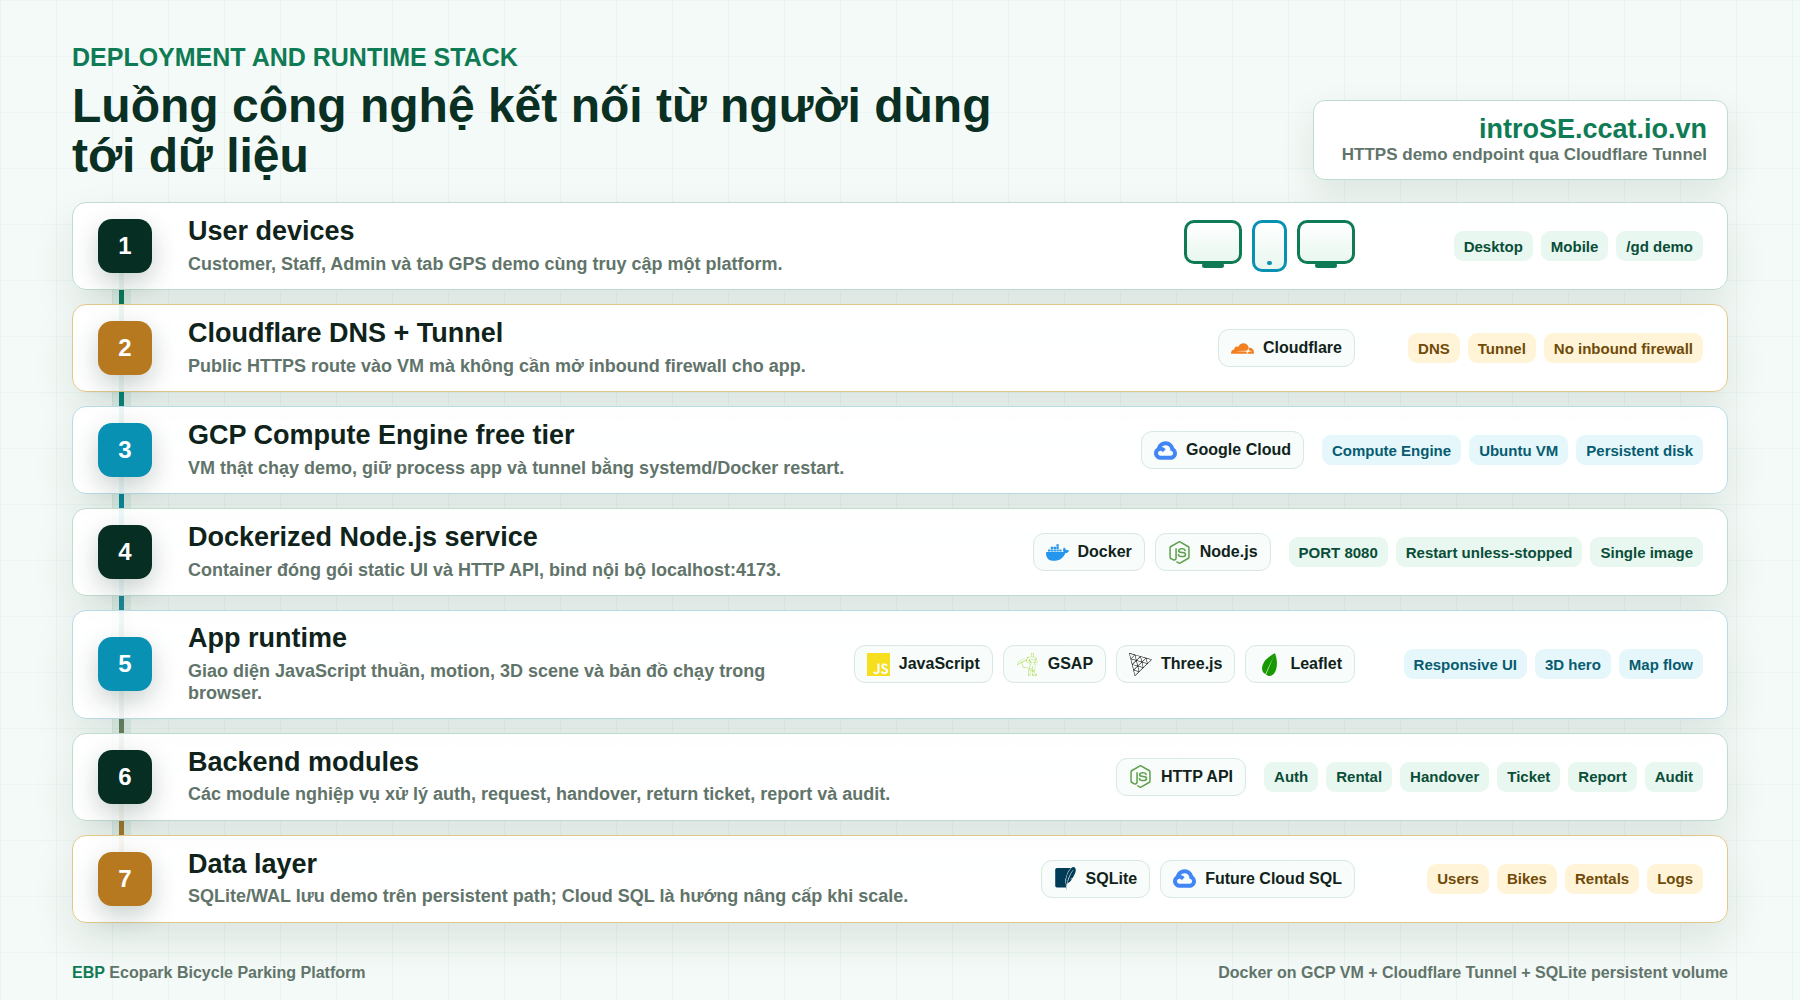
\includegraphics[width=\textwidth]{techstack/tech_stack_architecture.png}
\caption{Tech stack triển khai: Cloudflare Tunnel, GCP Compute Engine, Docker/Node.js và SQLite persistent volume}
\end{figure}

\begin{figure}[H]
\centering
\resizebox{\textwidth}{!}{%
\begin{tikzpicture}[
  box/.style={draw=EcoparkGreen,thick,rounded corners=2pt,fill=SoftGreen,minimum width=3.15cm,minimum height=1.05cm,align=center,font=\scriptsize},
  gcp/.style={draw=EcoparkTeal,thick,rounded corners=2pt,fill=cyan!8,minimum width=3.15cm,minimum height=1.05cm,align=center,font=\scriptsize},
  store/.style={draw=EcoparkAmber,thick,rounded corners=2pt,fill=yellow!10,minimum width=3.15cm,minimum height=1.05cm,align=center,font=\scriptsize},
  arr/.style={-{Latex[length=2.2mm]},thick,draw=Ink}
]
\node[box] (client) at (0,0) {Customer / Staff / Admin\\Browser UI};
\node[gcp] (vm) at (4.5,0) {GCP Compute Engine\\Docker/Node.js service};
\node[box] (domain) at (9,0) {Domain modules\\Auth, rental, pricing, reports};
\node[store] (sqlite) at (9,-2.0) {SQLite/WAL database\\users, bikes, rentals, logs};
\node[store] (disk) at (4.5,-2.0) {Persistent disk\\DB file and backup target};
\node[gcp] (secrets) at (4.5,1.9) {Secret Manager\\Runtime config};
\node[gcp] (logs) at (9,1.9) {Cloud Logging\\Monitoring and audit};
\node[box] (osm) at (0,-2.0) {OpenStreetMap tiles\\Optional map source};

\draw[arr] (client) -- (vm);
\draw[arr] (vm) -- (domain);
\draw[arr] (domain) -- (sqlite);
\draw[arr] (sqlite) -- (disk);
\draw[arr] (secrets) -- (vm);
\draw[arr] (vm) -- (logs);
\draw[arr] (client) -- (osm);
\end{tikzpicture}
}
\caption{Kiến trúc triển khai GCP với Node.js service và SQLite/WAL}
\end{figure}

\subsection{Đánh giá nhanh phần back-end}
Back-end hiện tại đã hỗ trợ vòng đời thuê-trả theo scope report: đăng ký/đăng
nhập, xác minh email bằng mã demo-local, reset mật khẩu demo-local, tách phiên
theo cookie, giữ chỗ xe bằng request pending, giao xe có cọc/giấy tờ, đổi xe
trước handover, trả xe khác bãi, tính vé, giảm giá cư dân, cập nhật trạng thái
xe, mở nhật ký audit và tổng hợp báo cáo có biểu đồ/table/CSV.

\begin{longtable}{P{0.22\textwidth}P{0.38\textwidth}P{0.30\textwidth}}
\toprule
\textbf{Mảng back-end} & \textbf{Đã có trong platform} & \textbf{GCP / production note} \\
\midrule
Authentication & Session cookie riêng cho từng browser/context; role customer, staff, admin; email verification, reset password và PBKDF2 salted password hash. & Secret Manager cho cấu hình; session store bền vững hơn nếu scale nhiều instance. \\
Rental lifecycle & Request pending, giữ xe, hủy/hết hạn, đổi xe trước handover, staff scope theo bãi, rental in-progress, return ticket. & SQLite/WAL đủ cho demo single-instance; Cloud SQL là hướng nâng cấp khi scale ngang. \\
Pricing & Bảng giá 1/2/3 giờ, phụ thu trễ block 30 phút, giảm cư dân 40\%. & Policy có thể versioning để đổi giá không sửa code. \\
Fleet reports & Chart doanh thu, trạng thái đội xe, lượt thuê/phụ thu, bảng chi tiết và CSV theo bộ lọc. & Có thể backup file SQLite định kỳ lên Cloud Storage nếu cần. \\
Auditability & Có bảng \texttt{BIKE\_STATUS\_LOGS}, API đọc log và panel nhật ký trạng thái xe. & Cloud Logging giữ log runtime; DB giữ audit nghiệp vụ. \\
Deployment & Codebase chạy local/demo và đã sẵn sàng đóng gói cho GCP Compute Engine bằng Node.js + SQLite. & Persistent disk giữ file DB; Cloud SQL chỉ cần khi nâng cấp production lớn hơn. \\
\bottomrule
\end{longtable}

\section{Component architecture and design}

\subsection{Phân tách component}
Thiết kế component được tổ chức theo tầng để giữ ranh giới rõ giữa giao diện,
API, logic nghiệp vụ và dữ liệu. Repo không tách microservice trong scope môn
học; thay vào đó, mỗi module giữ một trách nhiệm nhỏ và được kiểm tra bằng
unit/API test hoặc smoke test trình duyệt.

\begin{figure}[H]
\centering
\resizebox{\textwidth}{!}{%
\begin{tikzpicture}[
  layer/.style={draw=black!25,rounded corners=4pt,fill=black!2,minimum width=13.2cm,minimum height=1.25cm},
  label/.style={font=\scriptsize\bfseries,align=left},
  comp/.style={draw=EcoparkGreen,thick,rounded corners=2pt,fill=white,minimum width=2.65cm,minimum height=0.66cm,align=center,font=\scriptsize},
  arr/.style={-{Latex[length=2.0mm]},thick,draw=Ink}
]
\node[layer] (l1) at (0,0) {};
\node[label] at (-5.85,0.42) {Front-end};
\node[comp] (authui) at (-3.75,0) {Auth/Register};
\node[comp] (customerui) at (-1.20,0) {Customer rental};
\node[comp] (opsui) at (1.35,0) {Operations};
\node[comp] (gpsui) at (3.90,0) {\texttt{/gd} director};

\node[layer] (l2) at (0,-1.65) {};
\node[label] at (-5.85,-1.23) {HTTP/API};
\node[comp] (session) at (-2.55,-1.65) {Session + role guard};
\node[comp] (router) at (0,-1.65) {API router};
\node[comp] (static) at (2.55,-1.65) {Static/vendor};

\node[layer] (l3) at (0,-3.30) {};
\node[label] at (-5.85,-2.88) {Business};
\node[comp] (account) at (-2.55,-3.30) {Account service};
\node[comp] (rental) at (0,-3.30) {Rental service};
\node[comp] (fleet) at (2.55,-3.30) {Fleet/report service};

\node[layer] (l4) at (0,-4.95) {};
\node[label] at (-5.85,-4.53) {Data};
\node[comp] (db) at (-1.3,-4.95) {SQLite / WAL};
\node[comp] (logs) at (1.7,-4.95) {Status logs};

\draw[arr] (customerui.south) -- (router.north);
\draw[arr] (router.south) -- (rental.north);
\draw[arr] (rental.south) -- (db.north);
\draw[arr] (fleet.south) -- (logs.north);
\end{tikzpicture}
}
\caption{Component architecture theo tầng}
\end{figure}

\subsection{Luồng trạng thái thuê xe}
Luồng nghiệp vụ quan trọng nhất là vòng đời từ xe rảnh đến request, rental và
ticket. Thiết kế hiện tại chặn khách có nhiều rental đang chạy, chặn xe đã bị giữ
chỗ, và chỉ chuyển xe sang \textit{available} hoặc \textit{broken} sau khi Staff
hoàn tất trả xe.

\begin{figure}[H]
\centering
\resizebox{0.92\textwidth}{!}{%
\begin{tikzpicture}[
  state/.style={draw=EcoparkGreen,thick,rounded corners=2pt,fill=SoftGreen,minimum width=2.45cm,minimum height=0.78cm,align=center,font=\scriptsize},
  bad/.style={draw=EcoparkAmber,thick,rounded corners=2pt,fill=yellow!12,minimum width=2.45cm,minimum height=0.78cm,align=center,font=\scriptsize},
  arr/.style={-{Latex[length=2.0mm]},thick,draw=Ink}
]
\node[state] (available) at (0,0) {Available\\at station};
\node[state] (pending) at (2.9,0) {Pending\\pickup};
\node[state] (rented) at (5.8,0) {Rental\\in progress};
\node[state] (ticket) at (8.7,0) {Ticket\\completed};
\node[bad] (cancel) at (2.9,-1.55) {Cancelled\\or expired};
\node[bad] (broken) at (8.7,-1.55) {Broken\\not rentable};

\draw[arr] (available) -- (pending);
\draw[arr] (pending) -- (rented);
\draw[arr] (rented) -- (ticket);
\draw[arr] (pending) -- (cancel);
\draw[arr] (cancel.west) -| (available.south);
\draw[arr] (ticket) -- (broken);
\end{tikzpicture}
}
\caption{Lifecycle từ chọn xe đến xuất vé}
\end{figure}

\subsection{Sequence diagrams of implemented flows}

\begin{figure}[H]
\centering
\resizebox{\textwidth}{!}{%
\begin{tikzpicture}[
  actor/.style={font=\scriptsize\bfseries,align=center},
  lifeline/.style={draw=black!35,dashed},
  msg/.style={-{Latex[length=1.8mm]},draw=Ink,thick},
  note/.style={draw=EcoparkGreen,rounded corners=2pt,fill=SoftGreen,align=left,font=\tiny,inner sep=4pt}
]
\node[actor] at (0,0) {Customer};
\node[actor] at (4.2,0) {Customer UI};
\node[actor] at (8.4,0) {API Server};
\node[actor] at (12.6,0) {SQLite};
\foreach \x in {0,4.2,8.4,12.6} \draw[lifeline] (\x,-0.3) -- (\x,-6.2);

\draw[msg] (0,-0.8) -- node[above,font=\tiny] {1. filter station/type/range} (4.2,-0.8);
\draw[msg] (4.2,-1.45) -- node[above,font=\tiny] {2. \texttt{GET /api/stations}} (8.4,-1.45);
\draw[msg] (8.4,-2.1) -- node[above,font=\tiny] {3. station + inventory query} (12.6,-2.1);
\draw[msg] (8.4,-2.75) -- node[above,font=\tiny] {4. nearby stations + bikes} (4.2,-2.75);
\node[note] at (4.2,-3.25) {Map marker, station cards and bike cards\\show available/held states clearly};
\draw[msg] (0,-4.0) -- node[above,font=\tiny] {5. choose bike + duration} (4.2,-4.0);
\draw[msg] (4.2,-4.65) -- node[above,font=\tiny] {6. \texttt{POST /api/rental-requests}} (8.4,-4.65);
\draw[msg] (8.4,-5.3) -- node[above,font=\tiny] {7. create pending request} (12.6,-5.3);
\draw[msg] (4.2,-5.95) -- node[above,font=\tiny] {8. show request / cancel action} (0,-5.95);
\end{tikzpicture}
}
\caption{Sequence - Customer tìm bãi, chọn xe và gửi yêu cầu thuê}
\end{figure}

\begin{figure}[H]
\centering
\resizebox{\textwidth}{!}{%
\begin{tikzpicture}[
  actor/.style={font=\scriptsize\bfseries,align=center},
  lifeline/.style={draw=black!35,dashed},
  msg/.style={-{Latex[length=1.8mm]},draw=Ink,thick},
  note/.style={draw=EcoparkGreen,rounded corners=2pt,fill=SoftGreen,align=left,font=\tiny,inner sep=4pt}
]
\node[actor] at (0,0) {Staff/Admin};
\node[actor] at (4.2,0) {Operations UI};
\node[actor] at (8.4,0) {API Server};
\node[actor] at (12.6,0) {SQLite};
\foreach \x in {0,4.2,8.4,12.6} \draw[lifeline] (\x,-0.3) -- (\x,-6.8);

\draw[msg] (0,-0.8) -- node[above,font=\tiny] {1. verify identity + deposit} (4.2,-0.8);
\draw[msg] (4.2,-1.45) -- node[above,font=\tiny] {2. \texttt{POST /api/staff/handover}} (8.4,-1.45);
\draw[msg] (8.4,-2.1) -- node[above,font=\tiny] {3. create rental, mark rented} (12.6,-2.1);
\draw[msg] (8.4,-2.75) -- node[above,font=\tiny] {4. active rental} (4.2,-2.75);
\node[note] at (4.2,-3.25) {Return pipeline is enabled\\when a rental is active};
\draw[msg] (0,-4.0) -- node[above,font=\tiny] {5. return station/time/condition} (4.2,-4.0);
\draw[msg] (4.2,-4.65) -- node[above,font=\tiny] {6. \texttt{POST /api/staff/return}} (8.4,-4.65);
\draw[msg] (8.4,-5.3) -- node[above,font=\tiny] {7. ticket, bike update, audit log} (12.6,-5.3);
\draw[msg] (8.4,-5.95) -- node[above,font=\tiny] {8. ticket + charts + logs} (4.2,-5.95);
\draw[msg] (4.2,-6.55) -- node[above,font=\tiny] {9. issue ticket} (0,-6.55);
\end{tikzpicture}
}
\caption{Sequence - Staff handover, return và issue ticket}
\end{figure}

\subsection{End-to-end activity flow}
\begin{figure}[H]
\centering
\resizebox{\textwidth}{!}{%
\begin{tikzpicture}[
  actstep/.style={draw=EcoparkGreen,rounded corners=2pt,fill=SoftGreen,minimum width=3.20cm,minimum height=0.72cm,align=center,font=\scriptsize},
  sys/.style={draw=EcoparkTeal,rounded corners=2pt,fill=cyan!8,minimum width=3.20cm,minimum height=0.72cm,align=center,font=\scriptsize},
  staff/.style={draw=EcoparkAmber,rounded corners=2pt,fill=yellow!10,minimum width=3.20cm,minimum height=0.72cm,align=center,font=\scriptsize},
  arr/.style={-{Latex[length=1.8mm]},draw=Ink,thick}
]
\node[font=\bfseries] at (0,0.55) {Customer};
\node[font=\bfseries] at (4.2,0.55) {System};
\node[font=\bfseries] at (8.4,0.55) {Staff/Admin};

\node[actstep] (a1) at (0,0) {Đăng nhập / đăng ký};
\node[sys] (b1) at (4.2,0) {Validate account};
\node[actstep] (a2) at (0,-1.05) {Tìm bãi và chọn xe};
\node[sys] (b2) at (4.2,-1.05) {Check available + hold};
\node[actstep] (a3) at (0,-2.10) {Gửi request};
\node[staff] (c1) at (8.4,-2.10) {Kiểm tra request};
\node[staff] (c2) at (8.4,-3.15) {Nhận cọc/giấy tờ};
\node[sys] (b3) at (4.2,-3.15) {Create rental};
\node[actstep] (a4) at (0,-4.20) {Sử dụng xe};
\node[staff] (c3) at (8.4,-4.20) {Nhận xe trả};
\node[sys] (b4) at (4.2,-5.25) {Calculate ticket + update bike};
\node[staff] (c4) at (8.4,-5.25) {Xuất vé / xem report};

\draw[arr] (a1) -- (b1);
\draw[arr] (b1) -- (a2);
\draw[arr] (a2) -- (b2);
\draw[arr] (b2) -- (a3);
\draw[arr] (a3) -- (c1);
\draw[arr] (c1) -- (c2);
\draw[arr] (c2) -- (b3);
\draw[arr] (b3) -- (a4);
\draw[arr] (a4) -- (c3);
\draw[arr] (c3) -- (b4);
\draw[arr] (b4) -- (c4);
\end{tikzpicture}
}
\caption{Activity/swimlane flow cho demo end-to-end}
\end{figure}

\newpage
\section{Relational schema}

\subsection{Các quan hệ chính}
Lược đồ quan hệ dưới đây tập trung vào dữ liệu cần thiết cho 5 use case đã chọn. Ký hiệu: \textbf{PK} là khóa chính, \textbf{FK} là khóa ngoại.

\begin{longtable}{P{0.25\textwidth}P{0.65\textwidth}}
\toprule
\textbf{Bảng} & \textbf{Thuộc tính chính} \\
\midrule
\textbf{USERS} & \underline{user\_id} (PK), full\_name, phone, email, password\_hash, role, status, created\_at, last\_login\_at \\
\textbf{CUSTOMER\_PROFILES} & \underline{customer\_id} (PK, FK $\rightarrow$ USERS.user\_id), identity\_number, identity\_status, risk\_level, verified\_at \\
\textbf{VERIFICATION\_REQUESTS} & \underline{verification\_id} (PK), customer\_id (FK $\rightarrow$ CUSTOMER\_PROFILES.customer\_id), method, submitted\_data\_ref, verification\_status, reviewed\_by (FK $\rightarrow$ STAFF.staff\_id, nullable), rejected\_reason, created\_at, reviewed\_at \\
\textbf{WALLETS} & \underline{wallet\_id} (PK), customer\_id (FK $\rightarrow$ CUSTOMER\_PROFILES.customer\_id), balance, hold\_amount, wallet\_status, updated\_at \\
\textbf{WALLET\_TRANSACTIONS} & \underline{transaction\_id} (PK), wallet\_id (FK), type, amount, reference\_type, reference\_id, status, created\_at \\
\textbf{RENTAL\_PACKAGES} & \underline{package\_id} (PK), package\_name, package\_type, price, valid\_days, included\_minutes, overtime\_rate, active \\
\textbf{CUSTOMER\_PACKAGES} & \underline{customer\_package\_id} (PK), customer\_id (FK), package\_id (FK), starts\_at, expires\_at, remaining\_minutes, status \\
\textbf{STATIONS} & \underline{station\_id} (PK), station\_name, address, latitude, longitude, capacity, status \\
\textbf{BIKES} & \underline{bike\_id} (PK), station\_id (FK $\rightarrow$ STATIONS.station\_id), bike\_code, bike\_type, bike\_status, last\_maintenance\_at \\
\textbf{BIKE\_LOCKS} & \underline{lock\_id} (PK), bike\_id (FK $\rightarrow$ BIKES.bike\_id), lock\_status, firmware\_version, last\_sync\_at \\
\textbf{RIDES} & \underline{ride\_id} (PK), customer\_id (FK), bike\_id (FK), start\_station\_id (FK), end\_station\_id (FK), customer\_package\_id (FK, nullable), started\_at, ended\_at, ride\_status, duration\_minutes \\
\textbf{RIDE\_CHARGES} & \underline{charge\_id} (PK), ride\_id (FK $\rightarrow$ RIDES.ride\_id), base\_fee, package\_discount, overtime\_fee, penalty\_amount, total\_amount, settled\_at \\
\textbf{PAYMENTS} & \underline{payment\_id} (PK), transaction\_id (FK $\rightarrow$ WALLET\_TRANSACTIONS.transaction\_id), gateway\_transaction\_id, payment\_method, amount, payment\_status, paid\_at \\
\textbf{PENALTY\_RULES} & \underline{rule\_id} (PK), rule\_name, trigger\_condition, penalty\_amount, active \\
\textbf{PENALTIES} & \underline{penalty\_id} (PK), ride\_id (FK), rule\_id (FK), amount, reason, status, created\_at \\
\textbf{ISSUE\_REPORTS} & \underline{report\_id} (PK), bike\_id (FK), reported\_by (FK $\rightarrow$ USERS.user\_id), ride\_id (FK, nullable), issue\_description, report\_status, created\_at \\
\textbf{STAFF} & \underline{staff\_id} (PK, FK $\rightarrow$ USERS.user\_id), staff\_code, staff\_role, assigned\_area, active \\
\textbf{MAINTENANCE\_REQUESTS} & \underline{request\_id} (PK), report\_id (FK $\rightarrow$ ISSUE\_REPORTS.report\_id, nullable), bike\_id (FK), assigned\_to (FK $\rightarrow$ STAFF.staff\_id), priority, request\_status, repair\_note, created\_at, resolved\_at \\
\bottomrule
\end{longtable}

\subsection{Quan hệ giữa các bảng}
\begin{itemize}
  \item Một USERS có thể là một CUSTOMER\_PROFILES hoặc một STAFF tùy theo role.
  \item Một CUSTOMER\_PROFILES có thể có nhiều VERIFICATION\_REQUESTS theo thời gian; request gần nhất quyết định trạng thái xác thực hiện tại nếu quy trình cần duyệt lại.
  \item Một CUSTOMER\_PROFILES có đúng một WALLETS và có nhiều WALLET\_TRANSACTIONS.
  \item Một giao dịch nạp ví hoặc mua gói có thể được đối soát qua PAYMENTS và Payment Gateway.
  \item Một CUSTOMER\_PROFILES có thể sở hữu nhiều CUSTOMER\_PACKAGES theo thời gian; chỉ các gói còn hiệu lực mới được dùng khi thuê.
  \item Một CUSTOMER\_PROFILES có nhiều RIDES; mỗi RIDE dùng đúng một BIKE và có tối đa một CUSTOMER\_PACKAGES áp dụng.
  \item Mỗi RIDE có một RIDE\_CHARGES khi kết thúc chuyến; tổng tiền được trừ qua WALLET\_TRANSACTIONS.
  \item Một RIDE có thể phát sinh nhiều PENALTIES dựa trên PENALTY\_RULES.
  \item Customer có thể tạo ISSUE\_REPORTS, nhưng MAINTENANCE\_REQUESTS là luồng xử lý của Admin / Operator và Maintenance Staff.
\end{itemize}

\subsection{Ràng buộc nghiệp vụ quan trọng}
\begin{itemize}
  \item Không cho phép thuê xe nếu identity\_status chưa được xác thực hoặc wallet\_status không hoạt động.
  \item Tại một thời điểm, một Customer chỉ được có một RIDE ở trạng thái \textit{in\_progress}.
  \item Không cho phép UC003 nếu BIKES.bike\_status khác \textit{available} hoặc BIKE\_LOCKS.lock\_status không sẵn sàng.
  \item UC003 phải giữ một khoản tiền tối thiểu trong ví hoặc xác nhận gói ngày/tháng còn hiệu lực trước khi mở khóa xe.
  \item UC004 tính phí theo thời lượng thuê, áp dụng gói nếu hợp lệ, cộng overtime fee và penalty nếu vi phạm.
  \item Penalty không được miễn bởi gói ngày/tháng; nếu ví không đủ tiền, tài khoản chuyển sang trạng thái nợ hoặc bị tạm khóa thuê xe.
  \item Khi ISSUE\_REPORTS hoặc MAINTENANCE\_REQUESTS cho thấy xe không an toàn, BIKES.bike\_status phải chuyển sang \textit{maintenance}.
\end{itemize}

\newpage
\section{User interface design}

\subsection{Design direction}
Platform hiện thực các use case đã phân tích trong tài liệu này bằng một hệ
thống fullstack nhẹ, có profile local để demo nhanh và target triển khai GCP.
Front-end sử dụng HTML, CSS và JavaScript thuần; back-end sử dụng Node.js. Khi
deploy lên GCP, service Node.js được đặt trong VM/container và file SQLite/WAL nằm
trên persistent disk; khi chạy local, cùng SQLite schema được dùng để nhóm kiểm
thử end-to-end trên một máy nhưng vẫn thể hiện rõ luồng dữ liệu, trạng thái xe,
yêu cầu thuê, phiếu thuê và báo cáo vận hành.

Giao diện được thiết kế theo phong cách Civic Mobility Command Center: rail điều
hướng tối có thể cuộn tới từng vùng chức năng, workspace sáng, panel/form/table
sắc cạnh và mật độ thông tin phù hợp phần mềm điều phối vận hành. Bảng màu vẫn
bám chủ đề đô thị xanh Ecopark nhưng
không phụ thuộc vào một mảng xanh đơn điệu; các accent xanh nước và amber được
dùng để phân biệt trạng thái, bản đồ, loại xe và hành động chính. Lớp giao diện
được tinh chỉnh với thanh trên sticky dạng floating surface, session chip, menu
dropdown custom có trạng thái option rõ, trạng thái focus dễ nhận biết và bố cục
mobile tự trở về đầu trang khi chuyển màn hình làm việc. Thanh trên dùng nền gần
đặc, khoảng hở 14px và lớp mờ quanh mép để tách khỏi nội dung bên dưới mà không
làm rối khi cuộn hoặc mở dropdown. Giao diện cũng hỗ trợ ba chế độ \textit{Sáng}, \textit{Tối} và
\textit{Hệ thống}; theme được lưu ở trình duyệt, triển khai bằng design tokens
cho panel, bảng, dropdown và chart; bản đồ Leaflet có lớp xử lý màu riêng cho
dark mode còn scene Three.js giữ đủ tương phản để không mất khả năng quan sát khi demo. Trên mobile,
giao diện bỏ topbar riêng,
đưa scene 3D lên đầu hero, nén các metric thành một hàng ngang và rút rail điều
hướng tối thành dock icon-only nổi ở đáy màn hình, bao gồm cả refresh/theme/logout
để không cần một thanh topbar thứ hai. Ở desktop rộng, các panel có bảng dài như
\textit{Báo cáo \& CSV}, \textit{Yêu cầu nhận xe}, \textit{Danh sách trả xe} và
\textit{Đội xe} chiếm toàn bộ bề ngang workspace để chart và bảng không bị cắt.
Các dropdown ở bộ lọc báo cáo, nhận xe, trả xe, bãi trả và trạng thái đội xe
không dùng dropdown native của trình duyệt mà dùng cùng component custom có icon,
mô tả và trạng thái chọn; khi mở trong bảng, panel được nâng lớp z-index để menu
không bị cắt bởi panel kế tiếp. Chart tổng thu/phụ thu dùng cùng thang tiền với
chart doanh thu để so sánh tuần/tháng không bị lệch nghĩa và các thanh trạng thái
được bo tròn đồng nhất thay vì để phần màu bên trong thành hình chữ nhật.
Ở các viewport vận hành hẹp hoặc tablet/desktop nhỏ, hero staff/admin chuyển
sang một cột, dashboard chart giảm số cột và các bảng vận hành được chuyển thành
row-card có nhãn từng trường, nên báo cáo, yêu cầu nhận xe và đội xe vẫn đọc được
mà không cần kéo ngang trong panel. Phần đầu trang có một scene 3D nhỏ bằng
Three.js theo phong cách low-poly, mô phỏng Bike Hub isometric với đường nội khu,
bike lane, canopy, dock/rack, đèn trạng thái, hồ nước, bờ cỏ, dải cây xanh và ba
kiểu xe khác nhau. Bản scene mới mở rộng mặt hồ, bờ kè, cụm cây lớn quanh hồ và
hàng cây ven đường để phần minh hoạ có chiều sâu hơn trong khung hero hẹp. Scene
có thêm xe chạy vòng trên hành lang đường, người đi
bộ/kiểm tra xe/em nhỏ vẫy tay và sway cây nhẹ để tạo loop thị giác mượt. Scene
này dùng camera/frustum responsive để tự fit trong khung đăng nhập, hero dashboard
và mobile, thay cho cách phóng canvas bằng CSS; khi render lại cùng màn hình, app
giữ node canvas cũ để tránh nhấp nháy. Scene được đóng thành một dải preview cân
với cột nội dung ở màn hình đăng nhập và chỉ đóng vai trò nhấn thị giác, không
thay thế các bảng, form và trạng thái nghiệp vụ chính.

Các thẻ xe trong luồng khách hàng dùng minh hoạ SVG theo loại xe thay vì dùng
một icon chung cho mọi dữ liệu. City bike, Family tandem và Child-seat bike có
màu nhấn và hình dáng khác nhau để người dùng nhận biết loại xe nhanh hơn trước
khi gửi yêu cầu thuê. Card xe dùng bố cục ngang: minh họa loại xe ở cột trái, mã
xe, loại xe, trạng thái sẵn sàng và nút thuê gom ở cột phải để giảm khoảng trống
trong danh sách lựa chọn. Trên màn hình hẹp, hàng chọn thời lượng và nút thuê
được đưa xuống dùng toàn bộ bề ngang card để tránh bó chữ hoặc làm lệch viewport.
Khi xe không thuê được, card hiển thị rõ nguyên nhân như \textit{Chờ bạn nhận},
\textit{Bạn đang thuê}, \textit{Người khác giữ} hoặc \textit{Người khác thuê}
thay vì chỉ ghi chung là đang thuê.

Lớp chuyển động sử dụng GSAP cục bộ từ dependency npm. Các hiệu ứng vào trang được
gom bằng timeline, ưu tiên transform và opacity để giảm chi phí layout; các tương
tác nhỏ khi hover và toast cũng dùng GSAP với overwrite phù hợp. Giao diện tôn trọng
\texttt{prefers-reduced-motion}: khi người dùng giảm chuyển động, các hiệu ứng
được bỏ qua hoặc rút về trạng thái tĩnh. Các chi tiết giao diện đã được rà lại qua
các lượt chụp màn hình và tinh chỉnh, bao gồm bố cục màn hình đăng nhập, kích thước
hero trên mobile, độ dày bảng quản trị, vị trí toast, vị trí cuộn sau đăng nhập và cân
bằng giữa scene 3D với nội dung nghiệp vụ.

Màn hình khách hàng sử dụng bản đồ thật bằng Leaflet/OpenStreetMap để hiển thị
vị trí người dùng demo và marker các bãi xe Ecopark. Khách có thể dùng GPS demo
hoặc chuyển sang vị trí nhập tay, chọn phạm vi tìm kiếm, lọc loại xe bằng custom
dropdown HTML/CSS, chọn marker hoặc thẻ bãi để cập nhật danh sách xe sẵn sàng
tại bãi đó. Dropdown loại khách trong form đăng ký cũng dùng control custom thay
cho popup native của trình duyệt. Dropdown thời lượng trong card xe cũng dùng
cùng mẫu custom control, chỉ hiển thị nhãn giá ngắn trong trigger và mở menu có
mô tả đầy đủ khi cần chọn 1/2/3 giờ. Các dropdown vẫn giữ chiều rộng ổn định trên
desktop/mobile, không tạo scroll ngang và có trạng thái option đang chọn rõ ràng.
Khi không có bãi trong phạm vi đã chọn, giao diện hiển thị trạng thái rỗng rõ ràng để kích hoạt
alternative flow tìm kiếm thủ công/mở rộng phạm vi. Nếu tile bản đồ
không tải được trong môi trường offline, khung fallback nội bộ vẫn giữ pin bãi xe
để luồng nghiệp vụ không bị gián đoạn.

Workspace khách hàng gom vị trí tìm kiếm, bản đồ, bãi gần nhất, danh sách xe rảnh
và nút gửi yêu cầu vào cùng vùng \textit{Thuê xe}. Các vùng \textit{Lượt thuê}
và \textit{Tài khoản} được tách xuống dưới/ra rail điều hướng để màn đầu không
giống bảng quản trị thu nhỏ. Trạng thái GPS hoặc vị trí nhập tay được hiển thị
như chip overlay trong bản đồ, vì đây là ngữ cảnh của bản đồ thay vì một cảnh báo
riêng bên ngoài bộ lọc.

\subsection{Interface evidence}
Các hình dưới đây là screenshot trực tiếp từ platform hiện tại, dùng để chứng
minh UI đã có màn đăng nhập/đăng ký, workspace khách hàng trên desktop/mobile,
workspace vận hành và màn GPS hỗ trợ demo use case.

\begin{figure}[H]
\centering
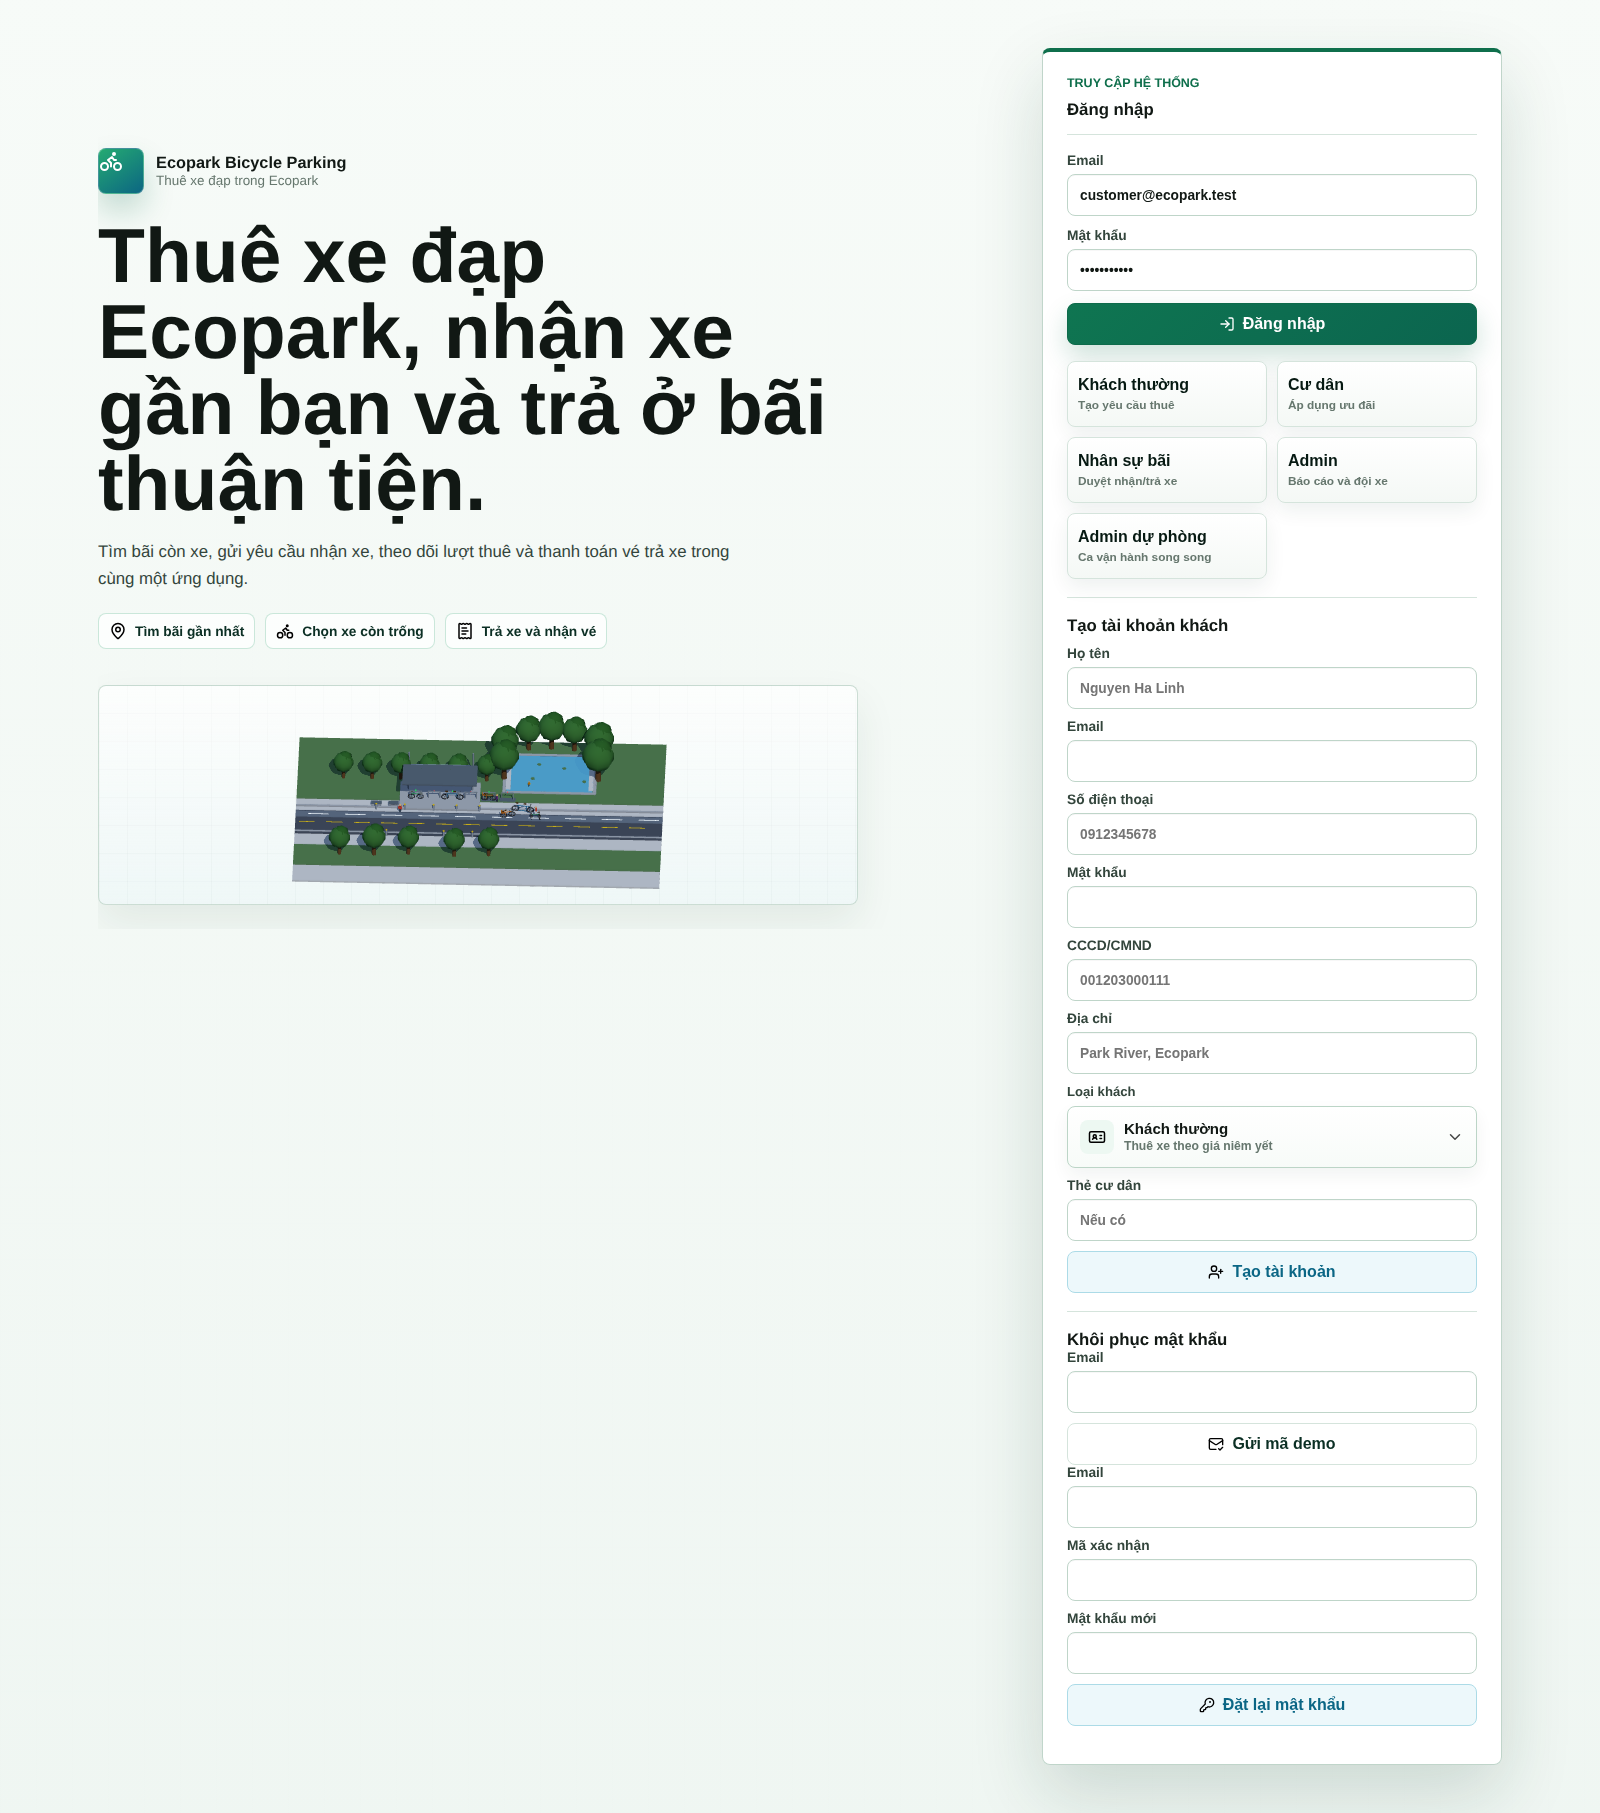
\includegraphics[width=0.92\textwidth,height=0.40\textheight,keepaspectratio]{auth_desktop.png}
\caption{Màn đăng nhập/đăng ký và 3D Bike Hub preview}
\end{figure}

\subsection{UC001 screen evidence}
Chuỗi ảnh dưới đây được chụp trực tiếp bằng script
\texttt{npm run screenshots:uc001}. Chuỗi này minh chứng basic flow UC001 và
alternative flow 1: hệ thống chặn form đăng ký khi thiếu thông tin bắt buộc,
hiển thị trường lỗi và giữ khách ở bước nhập liệu.

\begin{figure}[H]
\centering
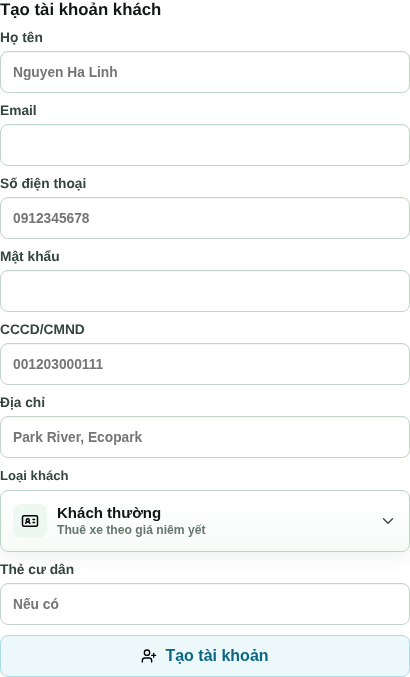
\includegraphics[width=0.48\textwidth,height=0.52\textheight,keepaspectratio]{uc001_flow/uc001_01_register_form.png}
\caption{UC001 bước 3: khách mở form tạo tài khoản với họ tên, email, số điện thoại, mật khẩu, CCCD/CMND, địa chỉ và loại khách}
\end{figure}

\begin{figure}[H]
\centering
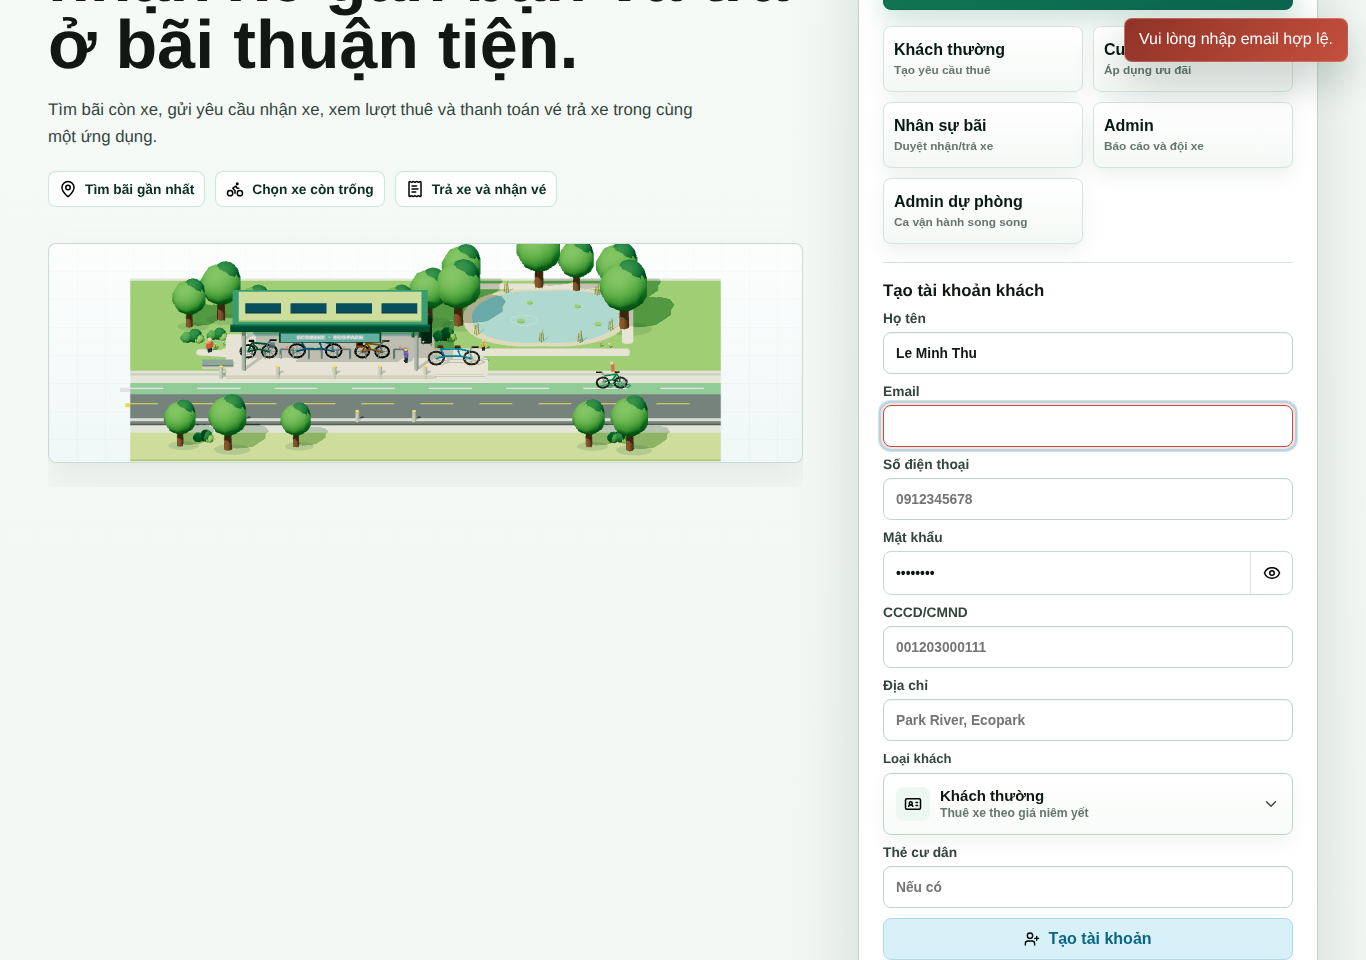
\includegraphics[width=0.92\textwidth,height=0.44\textheight,keepaspectratio]{uc001_flow/uc001_02_missing_required_fields.png}
\caption{UC001 alternative flow 1: thiếu email bắt buộc, UI giữ form tại bước nhập và hiển thị lỗi rõ ràng}
\end{figure}

\begin{figure}[H]
\centering
\begin{minipage}{0.31\textwidth}
\centering
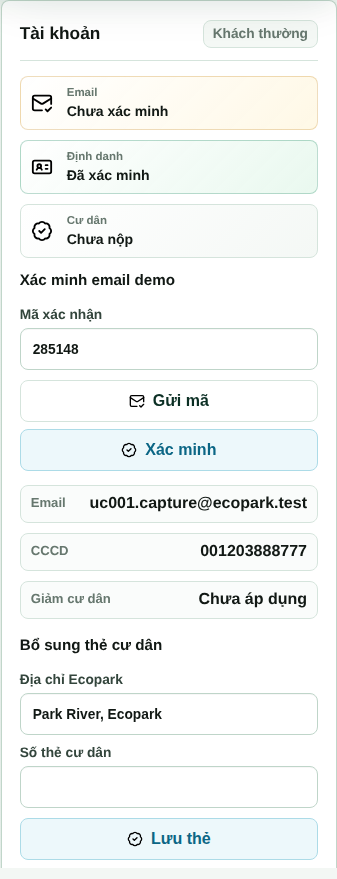
\includegraphics[width=\linewidth,height=0.42\textheight,keepaspectratio]{uc001_flow/uc001_03_account_created_unverified.png}\\
{\scriptsize Tài khoản tạo xong, email chưa xác minh}
\end{minipage}\hfill
\begin{minipage}{0.31\textwidth}
\centering
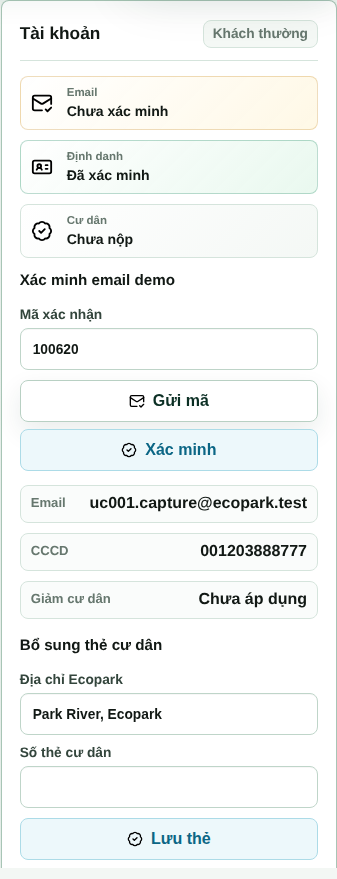
\includegraphics[width=\linewidth,height=0.42\textheight,keepaspectratio]{uc001_flow/uc001_04_email_code_ready.png}\\
{\scriptsize Mã xác minh demo-local được tạo trong platform}
\end{minipage}\hfill
\begin{minipage}{0.31\textwidth}
\centering
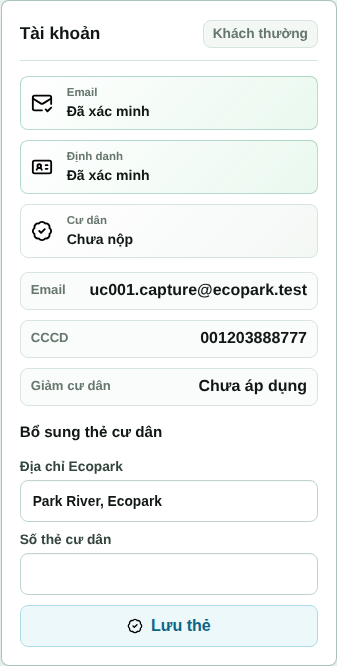
\includegraphics[width=\linewidth,height=0.42\textheight,keepaspectratio]{uc001_flow/uc001_05_email_verified.png}\\
{\scriptsize Email chuyển sang trạng thái đã xác minh}
\end{minipage}
\caption{UC001 bước 5--10: trạng thái tài khoản, mã xác minh email và hồ sơ đủ điều kiện thuê}
\end{figure}

\begin{figure}[H]
\centering

\includegraphics[width=0.92\textwidth,height=0.42\textheight,keepaspectratio]{customer_rent_desktop.png}
\caption{Workspace khách hàng: tìm bãi, bản đồ, chọn xe và gửi yêu cầu thuê}
\end{figure}

\clearpage
\begin{figure}[p]
\centering
\begin{minipage}{0.31\textwidth}
\centering
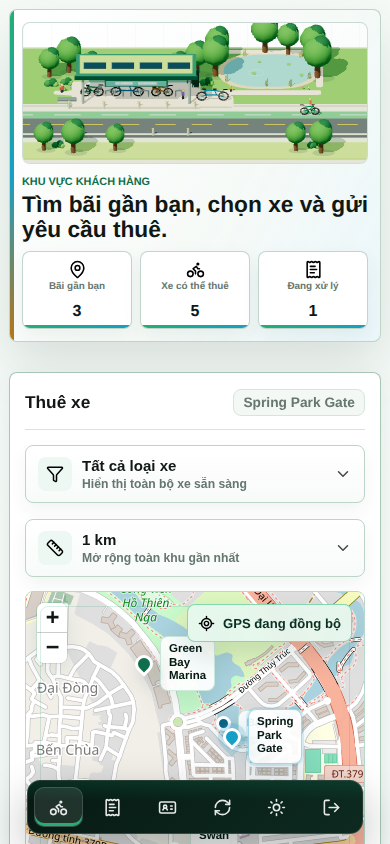
\includegraphics[width=\linewidth,height=0.58\textheight,keepaspectratio]{customer_mobile_overview.png}\\
{\scriptsize Tổng quan}
\end{minipage}\hfill
\begin{minipage}{0.31\textwidth}
\centering
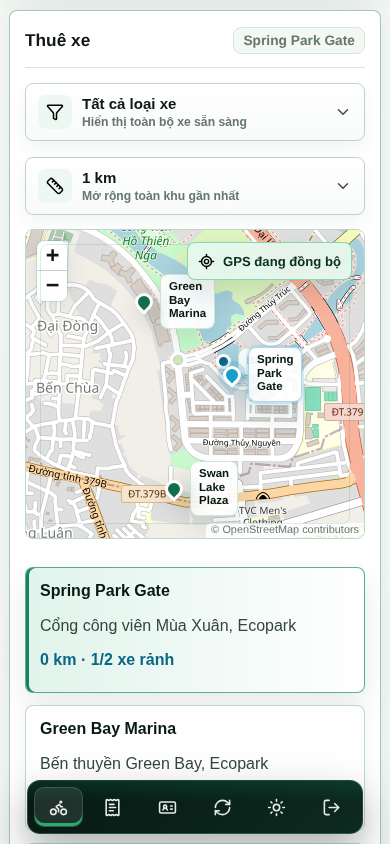
\includegraphics[width=\linewidth,height=0.58\textheight,keepaspectratio]{customer_mobile_search.png}\\
{\scriptsize Tìm bãi}
\end{minipage}\hfill
\begin{minipage}{0.31\textwidth}
\centering
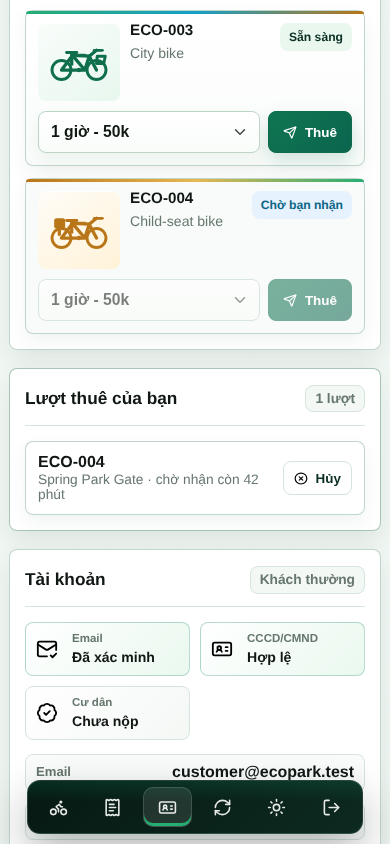
\includegraphics[width=\linewidth,height=0.58\textheight,keepaspectratio]{customer_mobile_bikes.png}\\
{\scriptsize Chọn xe}
\end{minipage}
\caption{UI điện thoại: 3D hero, metric compact, dock icon-only và luồng thuê xe}
\end{figure}
\clearpage

\begin{figure}[p]
\centering
\begin{minipage}{0.96\textwidth}
\centering
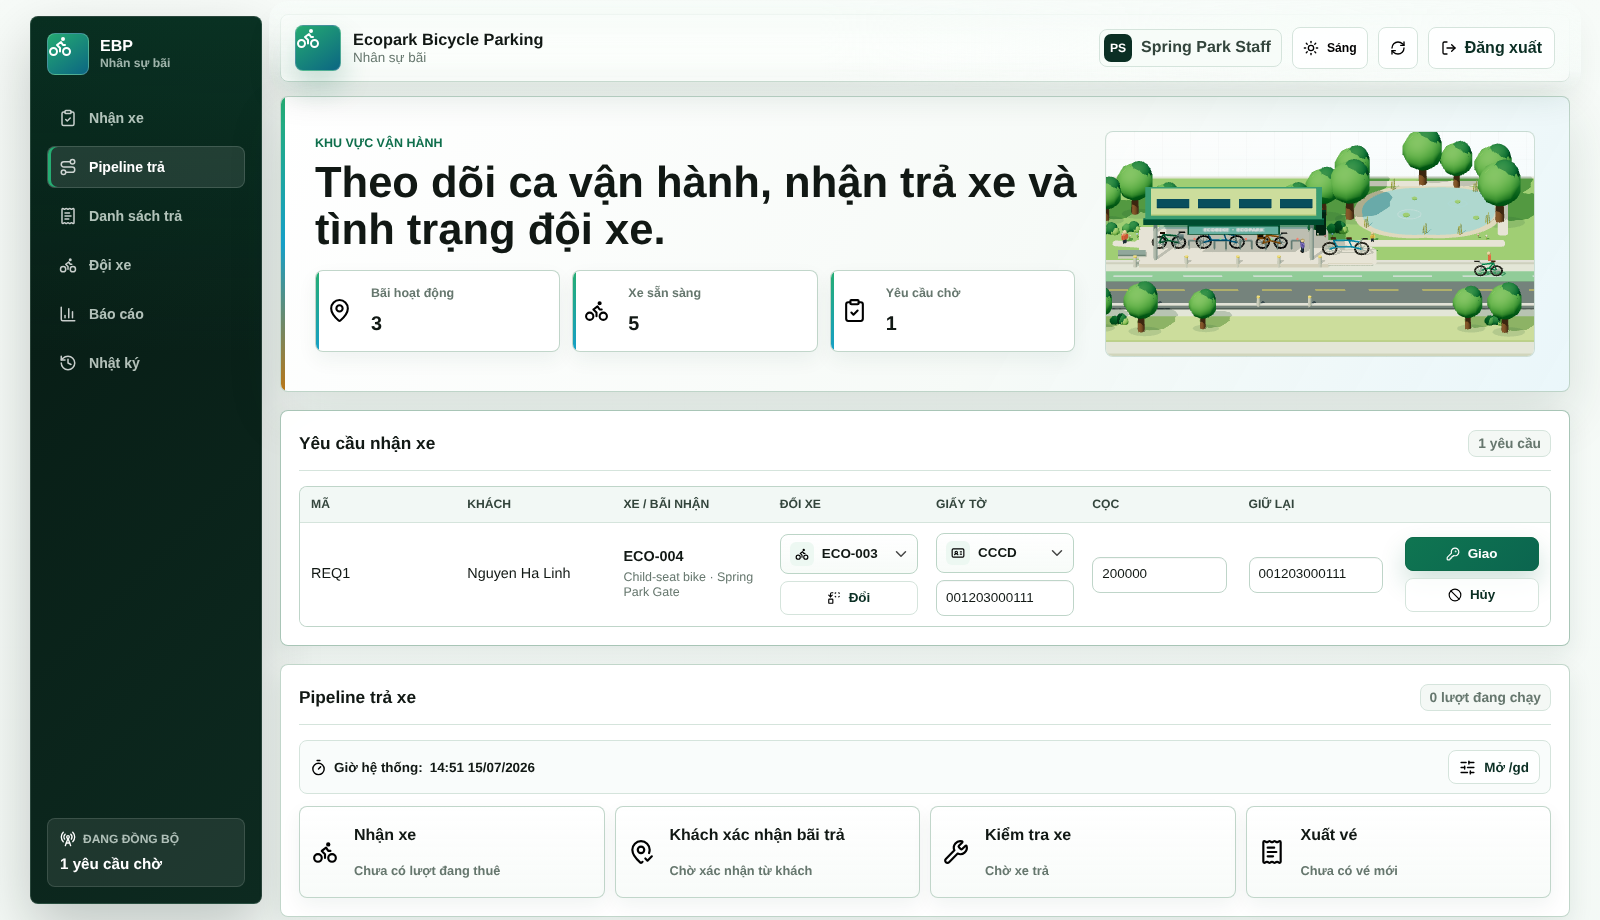
\includegraphics[width=\linewidth,height=0.32\textheight,keepaspectratio]{operations_overview.png}\\[2mm]
\raggedright{\small Tổng quan ca vận hành, yêu cầu nhận xe và pipeline trả xe}
\end{minipage}\\[4mm]
\begin{minipage}{0.96\textwidth}
\centering
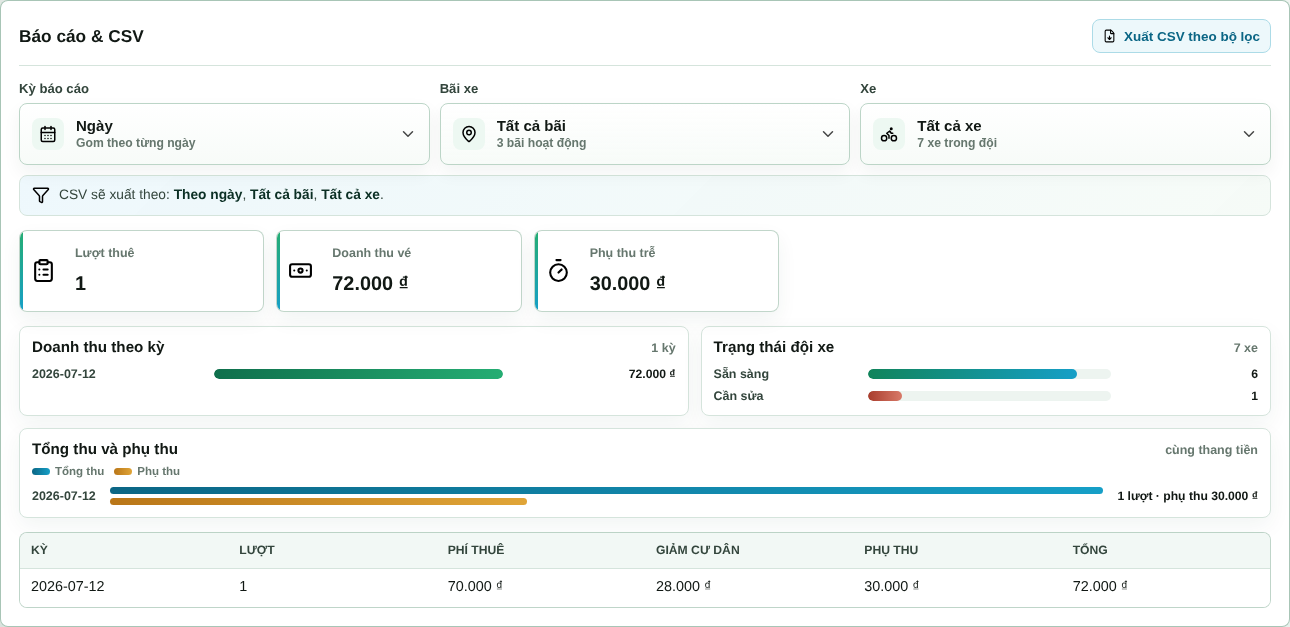
\includegraphics[width=\linewidth,height=0.32\textheight,keepaspectratio]{operations_report.png}\\[2mm]
\raggedright{\small Dashboard báo cáo, trạng thái đội xe và bộ lọc xuất CSV}
\end{minipage}
\caption{Workspace vận hành: nhận xe, trả xe, quản lý đội xe và báo cáo}
\end{figure}
\clearpage

\begin{figure}[H]
\centering

\includegraphics[width=0.86\textwidth,height=0.40\textheight,keepaspectratio]{gps_demo.png}
\caption{Route \texttt{/gd}: điều khiển GPS người dùng và đồng hồ hệ thống cho demo UC002/UC004}
\end{figure}

\subsection{UI screen-flow diagram}
\begin{figure}[H]
\centering
\resizebox{\textwidth}{!}{%
\begin{tikzpicture}[
  lane/.style={font=\footnotesize\bfseries,align=right,text=Ink},
  screen/.style={draw=EcoparkGreen,thick,rounded corners=2pt,fill=SoftGreen,minimum width=3.0cm,minimum height=0.82cm,align=center,font=\small,inner xsep=5pt},
  ops/.style={draw=EcoparkAmber,thick,rounded corners=2pt,fill=yellow!10,minimum width=3.0cm,minimum height=0.82cm,align=center,font=\small,inner xsep=5pt},
  aid/.style={draw=EcoparkTeal,thick,rounded corners=2pt,fill=cyan!8,minimum width=3.0cm,minimum height=0.82cm,align=center,font=\small,inner xsep=5pt},
  arr/.style={-{Latex[length=2.2mm]},draw=Ink,thick},
  support/.style={-{Latex[length=2.0mm]},draw=EcoparkTeal,thick,dashed}
]
\node[lane] at (0,1.60) {Customer};
\node[lane] at (0,0.15) {Staff/Admin};
\node[lane] at (0,-1.30) {Demo};

\node[screen] (authCustomer) at (2.35,1.60) {Login\\Register};
\node[screen] (rent) at (5.75,1.60) {Tìm bãi\\Chọn xe};
\node[screen] (history) at (9.15,1.60) {Lượt thuê\\Tài khoản};
\node[ops] (authStaff) at (2.35,0.15) {Login\\Register};
\node[ops] (pickup) at (5.75,0.15) {Nhận xe\\Giữ cọc};
\node[ops] (return) at (9.15,0.15) {Trả xe\\Xuất vé};
\node[ops] (manage) at (12.55,0.15) {Báo cáo\\Đội xe/Audit};
\node[aid] (director) at (2.35,-1.30) {\texttt{/gd}\\Demo director};
\node[aid] (gps) at (5.75,-1.30) {GPS người dùng\\theo đường};
\node[aid] (clock) at (9.15,-1.30) {Giờ hệ thống\\phụ thu};

\draw[arr] (authCustomer) -- (rent);
\draw[arr] (rent) -- (history);
\draw[arr] (authStaff) -- (pickup);
\draw[arr] (pickup) -- (return);
\draw[arr] (return) -- (manage);
\draw[support] (director) -- (gps);
\draw[support] (gps) -- (clock);
\end{tikzpicture}
}
\caption{Screen-flow chính của platform và route hỗ trợ demo GPS}
\end{figure}

Form đăng ký khách có gợi ý nhập liệu cho họ tên, số điện thoại, CCCD/CMND, địa
chỉ và nút hiện/ẩn mật khẩu để người dùng tự kiểm tra trước khi gửi. API đăng ký kiểm tra họ tên không chứa số/ký tự lạ, số điện thoại Việt Nam
dạng \texttt{0xxxxxxxxx} hoặc \texttt{+84xxxxxxxxx}, CCCD/CMND gồm 9 hoặc 12 chữ
số, đồng thời chặn số điện thoại hoặc giấy tờ định danh đã được dùng bởi tài
khoản khác. Theo UC001, CCCD/CMND hợp lệ là điều kiện tối thiểu trước khi thuê;
staff vẫn đối chiếu giấy tờ tại bước UC003 handover, còn trạng thái thẻ cư dân
pending/rejected chỉ ảnh hưởng ưu đãi cư dân chứ không chặn quyền thuê như khách thường.

Màn hình vận hành có pipeline trả xe riêng, luôn hiển thị bốn bước: nhận xe,
khách xác nhận bãi trả bằng GPS, kiểm tra tình trạng xe và xuất vé. Bảng chi
tiết bên dưới vẫn xử lý các input nghiệp vụ đầy đủ như bãi trả, giờ trả, tình
trạng xe và ghi chú kiểm tra, nhưng nút xuất vé chỉ mở khi customer đã xác nhận
vị trí trong bán kính bãi trả, giúp actor thấy rõ luồng UC004 ngay cả khi chưa
có rental active.

Để hỗ trợ trình bày use case trước lớp, ứng dụng có thêm route demo
\texttt{/gd}. Đây là demo director, không phải nghiệp vụ production mới: người
trình bày tìm/chọn từng tài khoản khách, chọn phiên khách đang chờ nhận xe hoặc
đang thuê xe khi có, chọn bãi đích, kéo thả marker GPS người dùng hoặc bấm snap
gần bãi. Hệ thống sẽ đưa marker về điểm gần nhất trên tuyến đường demo nội bộ và
hiển thị polyline đường đi tới bãi nhận/trả. Tọa độ sau khi snap hoặc kéo được
lưu theo từng customer qua API demo dùng chung. Khi marker \texttt{/gd} đang
chạy animation trên polyline đường, client stream các điểm trung gian theo
throttle, vì vậy tab khách hàng tương ứng đang chọn \texttt{GPS hiện tại} poll
cùng API và animate marker ``Bạn'', khoảng cách bãi và danh sách xe theo vị trí
đó thay vì chỉ nhảy tới điểm cuối. Khi chưa có lượt
active ở mode trả xe, UI vẫn cho kéo user đã chọn để chuẩn bị demo và hiển thị
empty state cho phần phiên UC. Cùng màn này có đồng hồ hệ thống nội bộ:
staff/admin có thể tua +15/+30/+60 phút hoặc reset về giờ thật để diễn trường
hợp quá hạn và phụ thu 30k/30 phút. Nhờ đó phần diễn UC002/UC004 không tạo cảm
giác xe bay thẳng qua hồ hoặc nhà, đồng thời phí phạt vẫn được tính bởi backend
theo cùng mốc giờ mà customer và staff nhìn thấy. Khi mở \texttt{/gd} trước lúc
danh sách tài khoản, bãi và phiên GPS sẵn sàng, giao diện hiển thị skeleton loading để không xuất hiện
một grid trắng trong lúc demo.

\subsection{Use-case to screen mapping}
\begin{longtable}{P{0.18\textwidth}P{0.34\textwidth}P{0.38\textwidth}}
\toprule
\textbf{Use case} & \textbf{Màn hình / chức năng web} & \textbf{Kết quả triển khai} \\
\midrule
UC001 & Đăng ký, đăng nhập, xác minh email, reset mật khẩu, hồ sơ khách, thẻ cư dân & Khách có tài khoản, CCCD/email/số điện thoại/địa chỉ, email đã xác minh, mật khẩu theo policy và trạng thái giảm giá cư dân nếu có thẻ hợp lệ. \\
UC002 & Danh sách bãi theo GPS demo/vị trí đã lưu/vị trí nhập tay, lọc loại xe, chọn xe, hủy request & Hệ thống hiển thị bãi trong phạm vi, số xe rảnh, trạng thái từng xe, tạo yêu cầu thuê với thời lượng 1/2/3 giờ ở mọi vị trí khách gửi và cho hủy request trước khi nhận xe. Vị trí hiện tại chỉ trở thành điều kiện bắt buộc ở bước handover. \\
UC003 & Bảng yêu cầu nhận xe cho Staff/Admin & Nhân sự được scope theo bãi, đối chiếu loại/số giấy tờ, nhận cọc 200k, ghi nhận giấy tờ giữ tại bãi, đổi sang xe rảnh cùng bãi khi cần, kiểm tra lại geofence khách ở bước handover, hủy yêu cầu không đủ điều kiện, tạo rental và chuyển xe sang trạng thái đang thuê; khi thao tác bị chặn, UI hiển thị lý do ngay trong panel nhận xe. \\
UC004 & Pipeline trả xe, bảng xe đang thuê và thao tác trả xe & Staff nhận xe tại bãi được phân công; Admin/Operator xử lý toàn hệ thống và hỗ trợ trả khác bãi. Customer phải xác nhận bãi trả bằng GPS trong bán kính bãi trước khi staff xuất vé; hệ thống tính phí thuê, chỉ giảm giá cư dân khi tài khoản là resident và thẻ cư dân verified, phụ thu trễ và hiển thị phiếu vừa xuất; nếu chưa đủ điều kiện xuất vé, UI hiện lý do thay vì chỉ khóa nút. \\
UC005 & Fleet table, quản lý bãi/xe, dashboard báo cáo, audit log & Admin/Operator quản lý bãi xe, xe, trạng thái xe, tra cứu vị trí xe, xem chart doanh thu/trạng thái đội xe/tổng thu và phụ thu, lọc thống kê bằng custom dropdown theo ngày/tuần/tháng, theo bãi/xe, xuất CSV và xem nhật ký đổi trạng thái. \\
\bottomrule
\end{longtable}

\section{Component implementation}

\subsection{Implemented modules}
\begin{longtable}{P{0.22\textwidth}P{0.28\textwidth}P{0.40\textwidth}}
\toprule
\textbf{Module} & \textbf{File chính} & \textbf{Vai trò triển khai} \\
\midrule
Frontend shell & \texttt{public/app.js}, \texttt{public/styles.css} & Render auth, customer, operations và \texttt{/gd}; quản lý state client, custom dropdown, map, table, form, report charts, audit timeline, demo clock, CSV download, inline operation errors và toast overlay không bị topbar che. \\
3D scene & \texttt{public/scene.js} & Mount scene Three.js low-poly, tự cleanup scene cũ, dùng frustum responsive và giữ \texttt{preserveDrawingBuffer} cho smoke test pixel. \\
API server & \texttt{server/app.js} & HTTP router, session cookie, role guard, static/vendor serving và các endpoint nghiệp vụ. \\
Database & \texttt{server/db.js} & SQLite schema, seed data, demo accounts, foreign keys và WAL mode; khi deploy GCP, file DB được đặt trên persistent disk. \\
Pricing & \texttt{server/pricing.js}, \texttt{server/app.js} & Tính phí cơ bản, phụ thu trễ và giảm giá cư dân theo policy đề bài; guard ticket-time yêu cầu customer\_type resident, cờ discount hợp lệ và resident card verified. \\
Backend tests & \texttt{test/app.test.js} & Test đăng ký, availability, resident discount guard, tạo request ngoài bán kính nhưng chặn handover theo GPS hiện tại, geofence return, handover, return ticket, reports và concurrent sessions. \\
Browser smoke tests & \texttt{scripts/ui-smoke.js}, \texttt{scripts/uc-flow-smoke.js} & Kiểm tra render UI, map/scene, overflow, console error, tab customer nhận marker GPS stream từ \texttt{/gd} và pipeline UC bằng Playwright. \\
\bottomrule
\end{longtable}

\subsection{Use-case implementation traceability}
\begin{longtable}{P{0.14\textwidth}P{0.30\textwidth}P{0.46\textwidth}}
\toprule
\textbf{UC} & \textbf{Component chính} & \textbf{Implementation note} \\
\midrule
UC001 & Auth UI, \texttt{registerCustomer}, \texttt{verifyEmail}, \texttt{resetPassword}, \texttt{submitResidentCard} & Custom customer-type dropdown, validation họ tên/phone/CCCD/password, PBKDF2 salted hash, email verification code, reset code, resident card verified/pending/rejected và blocked identity policy. \\
UC002 & Customer rental UI, station/bike APIs & Tìm bãi theo tọa độ hoặc vị trí đã lưu, chọn range/type, hiển thị held bike và tạo request pending pickup sau khi email/identity hợp lệ; API lưu tọa độ request nhưng chưa chặn theo bán kính bãi ở bước này. \\
UC003 & Pending request table, \texttt{handoverBike}, \texttt{exchangeRentalRequestBike} & Staff/Admin xác nhận giấy tờ, cọc 200k, scope request theo bãi nhân sự, kiểm tra GPS hiện tại của customer trước handover, đổi xe trước handover, tạo rental/deposit và đổi xe sang rented trong transaction; lỗi sai cọc/giấy tờ/bãi/bán kính được map thành thông báo tiếng Việt trong panel. \\
UC004 & Return pipeline, \texttt{confirmRentalReturn}, \texttt{returnBike}, pricing module & Customer xác nhận bãi trả trong bán kính bãi, staff nhận xe khác bãi khi đúng scope, tính ticket với resident discount guard tại thời điểm xuất vé, trả cọc, cập nhật bike station/status và ghi status log; nút xuất vé vẫn cho bấm khi chưa sẵn sàng để hiện lý do cần khách xác nhận. \\
UC005 & Fleet/report/audit panels, admin APIs & Quản lý bãi/xe, chặn sức chứa nhỏ hơn số xe, chặn đổi bãi xe đang thuê, lọc báo cáo bằng custom dropdown, hiển thị chart dùng cùng scale tiền, đọc audit log và export CSV. \\
\bottomrule
\end{longtable}

\section{API design and implementation}
Các API chính gồm nhóm xác thực, tra cứu bãi/xe, tạo yêu cầu thuê, giao xe, trả xe
và báo cáo. Dữ liệu được lưu trong SQLite/WAL theo các nhóm quan hệ đã nêu ở phần
\textit{Database design}; cùng DB này được dùng cho local demo và GCP deployment:
\begin{itemize}
  \item tài khoản và cư dân: USERS, CUSTOMER\_PROFILES, RESIDENT\_CARDS;
  \item bãi xe và đội xe: STATIONS, BIKE\_TYPES, BIKES;
  \item yêu cầu và lượt thuê: RENTAL\_REQUESTS, RENTALS;
  \item đặt cọc và vé thuê: RENTAL\_DEPOSITS, RENTAL\_TICKETS;
  \item truy vết vận hành và demo: BIKE\_STATUS\_LOGS, APP\_SETTINGS.
\end{itemize}

\subsection{API contract summary}
\begingroup
\small
\setlength{\tabcolsep}{4pt}
\begin{longtable}{P{0.12\textwidth}P{0.35\textwidth}P{0.16\textwidth}P{0.29\textwidth}}
\toprule
\textbf{Method} & \textbf{Endpoint} & \textbf{Role} & \textbf{Purpose} \\
\midrule
GET & \url{/api/session} & Public/session & Lấy user hiện tại từ session cookie. \\
POST & \url{/api/auth/register} & Public & Tạo tài khoản customer và hồ sơ định danh. \\
POST & \url{/api/auth/login} & Public & Đăng nhập và tạo session cookie. \\
POST & \url{/api/auth/logout} & Any session & Xóa session cookie hiện tại. \\
POST & \url{/api/auth/request-email-verification} & Customer & Tạo mã xác minh email demo-local, lưu dạng hash và thời hạn trong DB. \\
POST & \url{/api/auth/verify-email} & Customer & Xác minh email bằng mã demo-local trước khi gửi yêu cầu thuê. \\
POST & \url{/api/auth/request-password-reset} & Public & Tạo mã reset mật khẩu demo-local cho email active. \\
POST & \url{/api/auth/reset-password} & Public & Đặt lại mật khẩu theo policy và lưu hash PBKDF2 mới. \\
GET & \url{/api/bike-types} & Public & Lấy danh sách loại xe active. \\
GET & \url{/api/stations} & Public/customer & Lấy bãi xe, tồn kho tổng hợp và khoảng cách theo tọa độ. \\
GET & \url{/api/stations/:id/bikes} & Public/customer & Lấy xe trong bãi, trạng thái giữ chỗ và available. \\
GET & \url{/api/demo-clock} & Customer, Staff, Admin & Lấy giờ hệ thống nội bộ và mức phụ thu trễ cho demo. \\
POST & \url{/api/demo-clock} & Staff/Admin & Tua hoặc reset đồng hồ nội bộ dùng cho request, handover, return và audit log. \\
POST & \url{/api/rental-requests} & Customer & Tạo yêu cầu thuê xe pending pickup ở mọi vị trí khách gửi; vị trí được lưu để đối chiếu/fallback, còn điều kiện gần bãi được guard ở handover. \\
POST & \url{/api/rental-requests/:id/cancel} & Customer, Staff, Admin & Hủy request pending và giải phóng xe. \\
POST & \url{/api/staff/rental-requests/:id/exchange-bike} & Staff/Admin & Đổi request pending sang xe available cùng bãi trước handover. \\
GET & \url{/api/customer/history} & Customer & Lấy request, rental active, vé completed và request archive của khách. \\
POST & \url{/api/customer/rentals/:id/confirm-return} & Customer & Xác nhận bãi trả bằng tọa độ hiện tại trước khi staff xuất vé. \\
GET & \url{/api/gps-demo/users} & Public demo & Lấy danh sách tài khoản customer để \texttt{/gd} tìm và kéo GPS theo từng user. \\
GET & \url{/api/gps-demo/sessions} & Public demo & Lấy các phiên pending/active để \texttt{/gd} liên kết user với UC đang diễn. \\
GET / POST & \url{/api/gps-demo/position} & Public demo & Lưu/đọc tọa độ GPS demo theo từng customer giữa tab \texttt{/gd} và workspace khách hàng. \\
GET & \url{/api/staff/pending-requests} & Staff/Admin & Danh sách request chờ nhận xe. \\
POST & \url{/api/staff/handover} & Staff/Admin & Chuyển request thành rental sau khi xác nhận giấy tờ/cọc và kiểm tra GPS hiện tại của customer nằm trong bán kính bãi nhận. \\
GET & \url{/api/staff/active-rentals} & Staff/Admin & Danh sách rental đang chạy để xử lý trả xe. \\
POST & \url{/api/staff/return} & Staff/Admin & Trả xe sau xác nhận của customer, tính ticket, cập nhật vị trí/trạng thái xe. \\
GET & \url{/api/admin/bikes} & Staff/Admin & Tra cứu toàn bộ đội xe và trạng thái giữ chỗ. \\
GET & \url{/api/admin/reports} & Staff/Admin & Tổng hợp lượt thuê, doanh thu, phụ thu và fleet status. \\
GET & \url{/api/admin/bike-status-logs} & Staff/Admin & Đọc nhật ký đổi trạng thái xe, gồm mã xe, trạng thái cũ/mới, bãi, người đổi, lý do và thời gian. \\
POST & \url{/api/admin/users/:id/status} & Admin & Khóa/mở tài khoản để diễn account blocked alternative flow. \\
POST & \url{/api/admin/blocked-identities} & Admin & Thêm CCCD/CMND vào danh sách khóa vận hành. \\
DELETE & \url{/api/admin/blocked-identities/:identityNumber} & Admin & Gỡ CCCD/CMND khỏi danh sách khóa vận hành. \\
POST / PATCH & \url{/api/admin/stations} & Admin & Tạo/cập nhật bãi xe. \\
POST / PATCH & \url{/api/admin/bikes} & Admin & Tạo/cập nhật xe. \\
PATCH & \url{/api/admin/bikes/:id/status} & Staff/Admin & Đổi trạng thái xe kèm lý do và status log. \\
\bottomrule
\end{longtable}
\endgroup

Phiên đăng nhập được quản lý bằng session cookie riêng cho từng browser hoặc
browser context. Vì vậy khi trình bày, kịch bản thường có thể dùng một phiên
khách hàng, một phiên admin/operator và một tab \texttt{/gd} để kéo GPS người
dùng đang diễn và tua giờ hệ thống. Bộ smoke test vẫn kiểm tra mức tải demo tối đa gồm hai khách hàng,
hai tài khoản admin và một context \texttt{/gd}, bảo đảm các phiên không ghi đè
nhau. Seed demo cung cấp:
\begin{itemize}
  \item hai tài khoản khách: \texttt{customer@ecopark.test} và \texttt{resident@ecopark.test};
  \item hai tài khoản admin: \texttt{admin@ecopark.test} và \texttt{admin2@ecopark.test}.
\end{itemize}

Các quy tắc giá được triển khai đúng theo đề bài:
\begin{itemize}
  \item Giá cơ bản: 50k cho 1 giờ, 70k cho 2 giờ và 100k cho 3 giờ.
  \item Phụ thu trễ: 30k cho mỗi 30 phút phát sinh, làm tròn lên theo block 30 phút.
  \item Cư dân Ecopark hợp lệ được giảm 40\% trên phí thuê cơ bản.
  \item Tiền đặt cọc 200k và giấy tờ định danh được quản lý riêng, không tính là doanh thu vé thuê.
\end{itemize}

\section{Testing and evaluation}

\subsection{Local operation commands}
Repo cung cấp các lệnh vận hành chính:
\begin{itemize}
  \item \texttt{npm install}: cài dependency front-end/back-end.
  \item \texttt{npm run reset-db}: tạo lại SQLite database demo/local.
  \item \texttt{npm run dev}: chạy web app tại \texttt{http://127.0.0.1:4173}.
  \item \texttt{/gd}: mở demo director để kéo thả GPS người dùng theo tuyến đường demo và tua đồng hồ hệ thống.
  \item \texttt{npm run check}: kiểm tra cú pháp JavaScript cho app, server, test và script automation.
  \item \texttt{npm test}: chạy test nghiệp vụ back-end.
  \item \texttt{npm run test:coverage}: chạy test back-end kèm Node.js coverage report.
  \item \texttt{npm run smoke:ui}: kiểm tra render giao diện desktop/mobile bằng Playwright.
  \item \texttt{npm run smoke:uc}: chạy pipeline UI cho các luồng UC chính và một số alternative flow.
  \item \texttt{npm run screenshots:uc001}: sinh bộ ảnh UC001 và alternative flow 1 dùng trong report.
  \item \texttt{npm run docker:build}: kiểm tra container deployable cho target GCP.
\end{itemize}

\subsection{Test coverage}
\begin{longtable}{P{0.24\textwidth}P{0.36\textwidth}P{0.30\textwidth}}
\toprule
\textbf{Test layer} & \textbf{Coverage} & \textbf{Evidence/command} \\
\midrule
Backend API tests & Đăng ký, validation input, password policy, nâng cấp hash SHA-256 cũ sang PBKDF2, email verification, reset password, duplicate email/phone/CCCD, blocked identity, resident pending, stale resident-discount flag for visitor, held-bike availability, tạo request ngoài bán kính nhưng chặn handover theo GPS hiện tại, cancel request, exchange bike, staff station scope, geofence return, handover, capacity guard, return pricing, GPS demo theo từng customer, reports, audit logs, concurrent sessions. & \texttt{npm test} \\
Backend coverage & Coverage hiện tại theo Node.js built-in coverage: line 78.93\%, branch 69.31\%, functions 80.58\%. & \texttt{npm run test:coverage} \\
UI smoke tests & Auth/customer/admin trên 5 cỡ màn hình đại diện, GSAP load, Three.js canvas pixel, Leaflet marker, custom report dropdown, scale tiền của chart báo cáo, bảng vận hành rộng không scroll ngang, bảng vận hành hẹp dạng row-card, console error và horizontal overflow. & \texttt{npm run smoke:ui} \\
UC smoke tests & GPS context riêng, 2 customer + 2 admin sessions, chọn user trong \texttt{/gd} và kiểm marker customer map chạy theo, request/cancel/request again, staff handover, nhánh bấm xuất vé trước khi khách xác nhận để kiểm lý do bị chặn, customer confirm return, return ticket, chart dashboard, audit log và CSV report export. & \texttt{npm run smoke:uc} \\
Screenshot evidence & Bộ ảnh UC001 basic flow và alternative flow 1 được sinh từ chính app bằng Playwright. & \texttt{npm run screenshots:uc001} \\
CI/CD automation & GitHub Actions chạy static check, coverage, UI smoke, UC smoke và build Docker image deployable trên push/PR. & \texttt{.github/workflows/ci.yml} \\
Manual visual review & Screenshot auth, customer rental flow, operations workspace, mobile dock và GPS route. & Ảnh trong report UI section. \\
\bottomrule
\end{longtable}

Bộ test hiện kiểm tra đăng ký tài khoản, chống trùng email/phone/CCCD, chính
sách mật khẩu, nâng cấp hash cũ sang PBKDF2, xác minh email trước khi thuê,
reset mật khẩu demo-local, chặn CCCD/CMND bị khóa, thẻ cư dân pending thuê như
khách thường, loại xe đã giữ chỗ ra khỏi danh sách xe sẵn sàng, hủy yêu cầu
thuê và giải phóng xe, đổi xe trước handover, staff chỉ thấy/xử lý request đúng
bãi, chuyển yêu cầu thuê thành rental, chặn giảm sức chứa bãi dưới số xe hiện
có, tính vé trả xe có giảm giá cư dân/phụ thu trễ, sinh audit log trạng thái xe,
tổng hợp báo cáo và bốn phiên đăng nhập độc lập cho hai khách hàng cùng hai
admin.
Smoke test giao diện bằng Playwright mở các trạng thái desktop/mobile, kiểm tra
GSAP vendor đã tải, canvas Three.js có render, bản đồ Leaflet được mount với marker
thật, không phát sinh console error và không có tràn ngang ở cấp trang.
Smoke test UC mở demo director \texttt{/gd} ở context riêng, kiểm tra marker người dùng và trạng
thái đủ gần bãi trong kịch bản tải tối đa gồm bốn browser context cho hai khách
hàng và hai admin, đăng nhập bằng tài khoản cư dân, kiểm tra marker vị trí người
dùng, thử vị trí nhập tay ngoài phạm vi, gửi và hủy yêu cầu thuê, gửi lại yêu
cầu, đăng nhập Staff để giao xe và trả xe tại bãi được phân công, xuất ticket,
kiểm tra dashboard chart/audit log và tải báo cáo CSV; luồng trả khác bãi vẫn
được backend/UI hỗ trợ khi Admin/Operator xử lý toàn hệ thống.

\subsection{Evaluation and remaining limitations}
\begin{itemize}
  \item Sản phẩm đáp ứng đầy đủ 5 use case chính và các alternative flow quan
  trọng cần demo: GPS lỗi/nhập tay, hết xe trong phạm vi, hủy request, sai cọc/
  giấy tờ, trả khác bãi, xe hỏng và lọc báo cáo.
  \item Back-end đủ dùng cho demo/nộp môn học, đã dùng PBKDF2 salted password
  hash và mã xác minh/reset lưu dạng hash. Nếu chuyển production cần tích hợp
  dịch vụ gửi email thật, persistent session store, migration versioned và
  backup database.
  \item Dashboard vận hành đã có metric, chart doanh thu theo kỳ, phân bổ trạng
  thái đội xe, tổng thu/phụ thu cùng scale tiền, bảng chi tiết, CSV theo bộ lọc và audit timeline
  cho thay đổi trạng thái xe.
  \item Route \texttt{/gd} là công cụ thuyết trình để diễn vị trí người dùng theo đường
  và tua giờ nội bộ, không phải tracking GPS thật của thiết bị gắn trên xe hoặc điện thoại.
\end{itemize}


\end{document}
